%% Преамбула TeX-файла

% 1. Стиль и язык
\documentclass[14pt, utf8x]{G7-32} % Стиль (по умолчанию будет 14pt)

\usepackage[T2A]{fontenc}
\usepackage[russian]{babel}
\usepackage{setspace}
\usepackage{adjustbox}

% Остальные стандартные настройки убраны в preamble.inc.tex.
\sloppy

% Настройки стиля ГОСТ 7-32
% Для начала определяем, хотим мы или нет, чтобы рисунки и таблицы нумеровались в пределах раздела, или нам нужна сквозная нумерация.
\EqInChapter % формулы будут нумероваться в пределах раздела
\TableInChapter % таблицы будут нумероваться в пределах раздела
% \PicInChapter % рисунки будут нумероваться в пределах раздела

% Добавляем гипертекстовое оглавление в PDF
\usepackage[
bookmarks=true, colorlinks=true, unicode=true,
urlcolor=black,linkcolor=black, anchorcolor=black,
citecolor=black, menucolor=black, filecolor=black,
]{hyperref}

% Изменение начертания шрифта --- после чего выглядит таймсоподобно.
% apt-get install scalable-cyrfonts-tex

\IfFileExists{cyrtimes.sty}
    {
        \usepackage{cyrtimespatched}
    }
    {
        % А если Times нету, то будет CM...
    }

\usepackage{graphicx}   % Пакет для включения рисунков

% С такими оно полями оно работает по-умолчанию:
% \RequirePackage[left=20mm,right=10mm,top=20mm,bottom=20mm,headsep=0pt]{geometry}
% Если вас тошнит от поля в 10мм --- увеличивайте до 20-ти, ну и про переплёт не забывайте:
\geometry{right=15mm}
\geometry{left=30mm}

% Пакет Tikz
\usepackage{tikz}
\usetikzlibrary{arrows,positioning,shadows}

% Произвольная нумерация списков.
\usepackage{enumerate}

% ячейки в несколько строчек
\usepackage{multirow}

% itemize внутри tabular
\usepackage{paralist,array}


% Настройки листингов.
% 8 Листинги

\usepackage{listings}

% Значения по умолчанию
\lstset{
  basicstyle= \footnotesize,
  breakatwhitespace=true,% разрыв строк только на whitespacce
  breaklines=true,       % переносить длинные строки
%   captionpos=b,          % подписи снизу -- вроде не надо
  inputencoding=koi8-r,
  numbers=left,          % нумерация слева
  numberstyle=\footnotesize,
  showspaces=false,      % показывать пробелы подчеркиваниями -- идиотизм 70-х годов
  showstringspaces=false,
  showtabs=false,        % и табы тоже
  stepnumber=1,
  tabsize=4,              % кому нужны табы по 8 символов?
  frame=single
}

% Стиль для псевдокода: строчки обычно короткие, поэтому размер шрифта побольше
\lstdefinestyle{pseudocode}{
  basicstyle=\small,
  keywordstyle=\color{black}\bfseries\underbar,
  language=Pseudocode,
  numberstyle=\footnotesize,
  commentstyle=\footnotesize\it
}

% Стиль для обычного кода: маленький шрифт
\lstdefinestyle{realcode}{
  basicstyle=\scriptsize,
  numberstyle=\footnotesize
}

% Стиль для коротких кусков обычного кода: средний шрифт
\lstdefinestyle{simplecode}{
  basicstyle=\footnotesize,
  numberstyle=\footnotesize
}

% Стиль для BNF
\lstdefinestyle{grammar}{
  basicstyle=\footnotesize,
  numberstyle=\footnotesize,
  stringstyle=\bfseries\ttfamily,
  language=BNF
}

% Определим свой язык для написания псевдокодов на основе Python
\lstdefinelanguage[]{Pseudocode}[]{Python}{
  morekeywords={each,empty,wait,do},% ключевые слова добавлять сюда
  morecomment=[s]{\{}{\}},% комменты {а-ля Pascal} смотрятся нагляднее
  literate=% а сюда добавлять операторы, которые хотите отображать как мат. символы
    {->}{\ensuremath{$\rightarrow$}~}2%
    {<-}{\ensuremath{$\leftarrow$}~}2%
    {:=}{\ensuremath{$\leftarrow$}~}2%
    {<--}{\ensuremath{$\Longleftarrow$}~}2%
}[keywords,comments]

% Свой язык для задания грамматик в BNF
\lstdefinelanguage[]{BNF}[]{}{
  morekeywords={},
  morecomment=[s]{@}{@},
  morestring=[b]",%
  literate=%
    {->}{\ensuremath{$\rightarrow$}~}2%
    {*}{\ensuremath{$^*$}~}2%
    {+}{\ensuremath{$^+$}~}2%
    {|}{\ensuremath{$|$}~}2%
}[keywords,comments,strings]

% Подписи к листингам на русском языке.
\renewcommand\lstlistingname{\cyr\CYRL\cyri\cyrs\cyrt\cyri\cyrn\cyrg}
\renewcommand\lstlistlistingname{\cyr\CYRL\cyri\cyrs\cyrt\cyri\cyrn\cyrg\cyri}


% Полезные макросы листингов.
% Любимые команды
\newcommand{\Code}[1]{\textbf{#1}}


\begin{document}

% Исправляем нумерацию страниц
\setcounter{page}{2}

% Исправляем абзацный отступ
\setlength{\parindent}{1.25cm}

\frontmatter % выключает нумерацию ВСЕГО; здесь начинаются ненумерованные главы: реферат, введение, глоссарий, сокращения и прочее.

% Команды \breakingbeforechapters и \nonbreakingbeforechapters
% управляют разрывом страницы перед главами.
% По-умолчанию страница разрывается.

% \nobreakingbeforechapters
% \breakingbeforechapters

\chapter*{Аннотация}

% Объем аннотации должен составлять не более 1500 знаков. В аннотации необходимо
% отразить:
% - цели и задачи работы;
% - полученные результаты;
% - рекомендации, предложенные на основании данной работы.

Целью данной работы является разработка алгоритма переноса стиля из неформального стиля, присущего интернет общению, в стиль формальный и наоборот.

В ходе выполнения исследования был собран параллельный набор данных из 18 тысяч параллельных пар предложений неформальный-формальный стиль.
В основе набора данных лежит корпус текстов статей с сайта Луркморье.
Для разметки данных были привлечены студенты-лингвисты из Российского Государственного Гуманитарного Университета.

В работе были исследованы 4 различных метода, как основанные на полном отсутствии параллельных данных, так и с привлечением современных языковых моделей.
Подходы, основанные на использовании больших языковых моделей, оказались наиболее эффективными для решения поставленной задачи.
Данные методы, совместно с параметро-эффективными методами обучения, не требуют наличия большого количества параллельных данных, а с увеличением количества параметром языковой модели, объём необходимого количества данных для дообучения сводится до минимума.


\tableofcontents

\Abbreviations %% Список обозначений и сокращений в тексте
В настоящем отчете о НИР применяют следующие сокращения и обозначения

\begin{description}
\item[кол-во] количество
\item[РГГУ] Российский Государственный Гуманитарный Университет
\item[VAE] variational auto-encoder
\item[DAE] denoising auto-encoder
\item[LLM] Large Language Models
\item[GPT] Generative pre-trained transformer
\item[PEFT] Parameter-Efficient Fine-Tuning
\item[LoRA] Low-Rank Adaptation of Large Language Models

\end{description}


\Introduction
% Введение содержит четкое и краткое обоснование выбора темы, ее актуальности, определение
% объекта и предмета исследования, целей и задач, перечень методов исследования; краткую
% формулировку научно-теоретической и практической значимости исследования; сведения об
% апробации результатов исследования (публикации, выступления на конференциях и т.д.).

% Объектом исследования является перенос стиля текста.
% Предметом исследования являются архитектурные особенности нейронных сетей.

% Теоретическая значимость работы заключается в 

% Практическая -- результаты исследования могут быть использованы для повышения качества переноса.

% С ростом популярности больших генеративных языковых моделей, управление его генерацией является
% В последние годы исследования стиля текста привлекают внимание не только лингвистов, но и многих исследователей в области компьютерных наук.
% В частности, исследователи компьютерных наук исследуют задачу переноса стиля текста, которая становится все более популярной ветвью генерации естественного языка, целью которой является изменение стилистических свойств текста при сохранении его независимого содержания стиля.

% В последние годы в компьютерной лингвистике исследуют задачу переноса стиля текста, которая становится все более популярной ветвью генерации естественного языка, целью которой является изменение стилистических свойств текста при сохранении его независимого содержания стиля.

Возможность управлять стилем текста является очень актуальной и важной задачей, потому что это делает обработку естественного языка более ориентированной на пользователя.
Алгоритмы переноса стиля текста имеют множество непосредственных применений.
Например, одним из таких приложений являются интеллектуальные боты, для которых
пользователи предпочитают эмоциональную и последовательную персону.
Другим применением является разработка интеллектуальных помощников по написанию текстов;
например, авторам-неспециалистам часто требуется улучшить свои тексты, чтобы они лучше соответствовали их назначению, например, более профессиональному, вежливому, объективному, с чувством юмора или другим продвинутым требованиям к письму, на освоение которых могут потребоваться годы опыта.
Другие приложения включают автоматическое упрощение текста, увеличение объективности онлайн-текста, борьбу с оскорбительными выражениями и токсичными высказываниями и т.д.

% Данная задача, хоть и напоминает другие проблемы компьютерной лингвистики, например, машинный перевод или парафраз, является более сложной в связи с отсутствием достаточного объёма параллельных данных.
Данная задача близка к другим задачам компьютерной лингвистики, например, машинному переводу или парафразу.
Поэтому методы и экспертиза, накопленные в решении этих проблем, могут применяться и для неё.

Для выполнения поставленной цели, необходимо решить следующие задачи:
\begin{itemize}
    \item проанализировать текущее состояние исследуемой области, существующие подходы к решению данной или схожей задачи, имеющиеся наборы данных;
    \item определить необходимые метрики и критерии оценки качества будущего алгоритма;
    \item собрать собственный набор данных;
    \item провести эксперименты для проверки работоспособности выбранных методов на собранном наборе данных;
    \item сделать выводы на основании полученных результатов;
    \item сформулировать планы для дальнейшего развития исследования.
\end{itemize}


\mainmatter % это включает нумерацию глав и секций в документе ниже

\chapter{Анализ проблемы} \label{cha:analysis}

\section{Постановка задачи} \label{cha:analysis:sec:target}
Задачей работы является разработка модели перевода текста формально-нейтрального стиля в стиль неформальный, присущий стилю интернет-общения, например, подобного в интернет-энциклопедии Луркморье. И наоборот: из неформального в формальный.

Свести эту задачу к классическим методам машинного перевода трудно, потому что не существует подобного параллельного корпуса на русском языке достаточного объёма и собрать его самостоятельно крайне сложно.
Однако, параллельный корпус небольшого объёма (от 10 тысяч предложений) необходим. Во-первых, нужно оценить результаты работы будущей модели, например, с помощью BLUE score. Во-вторых, существуют методы обучения с учителем, не требующие больших объёмов данных и они будут исследованы в данной работе.

\section{Понятие стиля текста}
В рамках данной задачи можно выделить два определения стиля:
\begin{enumerate}
    \item \textbf{Лингвистическое}. Стиль -- это интуитивное понятие, которое включает в себя способ передачи некоторой семантики \cite{mcdonald-pustejovsky-1985-computational}. 
    Семантика (или "`содержание"') текста относится к предмету или аргументу, который автор хочет донести.
    Стиль текста -- это литературный элемент, который описывает способы использования автором языка, включая выбор слов, структуру предложения, образный язык и расположение предложений, и работает вместе для создания тона, образа и семантики в тексте. Стиль указывает на то, как автор описывает события, объекты и идеи. С помощью стиля автор может предоставить дополнительную информацию, которую читатель сможет интерпретировать и на которую может реагировать.
    Невозможно перечислить все возможные стили. Каждый человек обладает уникальным набором приемов, часто адаптированных к конкретным людям, для достижения своих межличностных целей.
    \item \textbf{Основанное на данных} (используемое в исследованиях по переносу стиля текста) -- часто исследователи рассматривают "`стиль"' как атрибуты текста, зависящие от корпусов, принадлежащих конкретному стилю. Эти специфичные корпуса обычно содержат стилистические атрибуты, которые нетрудно смоделировать с помощью методов машинного обучения \cite{jin2021deep}.
\end{enumerate}

\section{Метрики качества} \label{cha:analysis:sec:metrics}
Качество переноса стиля принято оценивать по трём параметрам:
выраженность стиля (поменялся ли стиль в сгенерированном предложении, как этого требовалось),
сохранение смысла (сохранилась ли семантика исходного предложения) и плавность текста (text fluency, насколько хорошо сгенерированное предложение соответствует грамматике и нормам языка) \cite{briakou2021evaluating}.
Помимо автоматических метрик для оценки указанных параметров, распространённым является использование человеческого труда для оценки качества.

\subsection{Выраженность стиля}
Для автоматической оценки выраженности стиля большинство исследователей обучают классификатор, который определяет имеет ли сгенерированное предложение желаемые стилистические атрибуты \cite{jin2021deep}.
Общее качество определяется как соотношение количества правильно классифицированных предложений к общему числу предложений в тестовом наборе данных. Чем выше значение, чем лучше модель переносит стиль. 
Стоит отметить, что данная метрика не всегда показывает реальное качество алгоритма, так как оценки классификатора могут не коррелировать с человеческими оценками \cite{li2018delete}.

\subsection{Сохранение семантики текста}
Чтобы количественно измерить объем оригинальной семантики, сохраняемой после операции переноса стиля, применяются автоматические метрики, которые хорошо зарекомендовали себя в других задачах генерации естественного языка:
\begin{itemize}
    \item BLEU \cite{bleu}, sacreBLEU \cite{sacrebleu} -- изначально была создана для оценки качества машинного перевода. Это первая метрика, которая показала высокую корреляцию между человеческими оценками и качеством переведённого текста \cite{hu2023text}.
    Для её подсчёта сгенерированный текст сравнивается с набором заранее подготовленных высококачественных референсов.
    Однако, у этой метрики есть определённый набор недостатков.
    Во-первых, в задаче переноса стиля текста простое копирование предложения может дать высокую оценку, потому что большое количество n-грамм часто переиспользуется в парафразе \cite{jin2021deep}.
    Во-вторых, некоторые исследования показывают, что метрика может показывать низкую корреляцию с человеческими оценками \cite{li2018delete, mir2019evaluating}.
    В-третьих, обязателен параллельный набор данных для оценки, что не всегда имеется;
    \item source-BLEU/self-BLEU -- в связи с тем, что параллельный набор данных часто недоступен, а метрика BLEU подразумевает его наличие, исследователи используют его модификацию, в которой переписанное предложение сравнивается с исходным предложением. Интуиция заключается в предположении, что семантика предложения сохраняется и перефразированное предложение будет иметь много совпадающих n-грамм с исходным предложением;
    \item METEOR \cite{meteor} -- оценивает сгенерированное предложение, сопоставляя его с одним или несколькими референсами. Сравнение основано на точном совпадении слов и фраз, основ слова (стемах), синонимах и перефразировках. Метрика рассчитывается как среднее гармоническое значение точности (precision) униграммы и полноты (recall), при этом полнота взвешивается выше;
    \item ROUGE-L \cite{lin-2004-rouge} -- метрика, ориентированная на полноту (recall), созданная для оценки суммаризации текста, в которой используется концепция самой длинной общей подпослдеовательности (Longest Common Subsequence, LCS). Интуиция, лежащая в основе данной метрики, подразумевает, что чем длинее LCS между двумя предложениями, тем больше они схожи. Оценка равна 1, когда два предложения равны, и 0, в противоположном случае;
    % \item chrF --
    % \item Word Mover Distance (WMD) --
    \item Cosine Similarity, BERTScore и пр. -- вычисляется косинусная близость эмбеддингов между сгенерированным и референсным предложениями \cite{fu2017style, zhang2020bertscore}. Подразумевается, что эмбеддинги сгенерированного и референсного предложения должны иметь близкое расстояние, чтобы сохранить семантику;
    \item и другие.
\end{itemize}

\subsection{Плавность текста}
Плавность текста является основным требованием к генерациям на естественном языке.
Для оценки плавности используется метрика перплексии, которая вычисляется с помощью языковой модели, предварительно обученной на желаемом наборе данных \cite{yang2019unsupervised}.

% TODO можно написать подробнее про подсчет метрики, упомянуть Kneser-Ney и GPT

Однако, эффективность перплексии до сих пор остаётся спорным вопросом. Некоторые исследования \cite{pang2019unsupervised} показывают её высокую корреляцию с человеческими оценками, в то время как другие \cite{mir2019evaluating} утверждают, что значительная корреляция отсутствует.

Перплексия, полученная с помощью языковой модели, может иметь следующие нежелательные свойства \cite{jin2021deep}:
\begin{itemize}
    \item Склонность оценивать выше более короткие предложения, чем длинные;
    \item Имея одинаковое значение, менее частые слова будут оцениваться ниже, чем частые;
    \item Качество языковой модели очень сильно влияет на метрику. Оценки перплексии, зависят от учебного корпуса, архитектуры и конфигурации языковой модели, а также конфигурации оптимизации. Следовательно, генерации различных парафразеров должны оцениваться с помощью точно такой же языковой модели для объективного сравнения, что усложняет оценку качества.
\end{itemize}

\subsection{Человеческая оценка}
Существует несколько способов провести ручную оценку качества.
Выделяют точечную и попарную оценки. В первом случае у асессора запрашивается абсолютная оценка результатов генерации модели, а в последнем случае оценивается какая из нескольких генераций лучше или просится ранжирование. Так же человек помимо общей оценки, может отдельно оценить качество переноса стиля, качество сохранения семантики и плавность текста.

Однако, человеческая оценка дорога и трудновоспроизводима.
Использование ручного труда требует большого количества времени и финансовых вложений.
Помимо этого, человеческие оценки, полученные в разных исследованиях часто нельзя сравнить напрямую, потому что они могут быть субъективными и невоспроизводимыми \cite{belz-etal-2020-reprogen}.
Некоторые стили очень сложно оценить без экспертизы и предварительной подготовки.



\section{Наборы данных} \label{cha:analysis:sec:datasets}
Задача переноса стиля достаточна обширна.
Выделяют следующие подзадачи: изменение формальности, вежливости, токсичности, сентимента и пр.
Данная работа фокусируется на изменении формальности текста, поэтому рассмотрению подлежат существующие наборы данных для этой задачи.

Изменение формальности это один из наиболее отличительных стилистических аспектов, который можно наблюдать во многих лингвистических явлениях, таких как  полные имена вместо аббревиатур или сокращений, присутствие сленга и просторечий и пр.
На текущий момент существует лишь несколько параллельных наборов данных для этой задачи. Самые популярные из них это англоязычный Grammarly’s Yahoo Answers Formality Corpus (GYAFC) \cite{gyafc} и мультиязычный (Итальянский, Французский и Португальский) XFORMAL \cite{xformal}.
К сожалению, на русском языке отсутствуют параллельные наборы данных, состоящие из пар формальное-неформальное предложение.
Поэтому набор данных придётся собирать самостоятельно.

% Надо ставить задачу переноса из неформального в формальный, потому что это все представляют как выглядит формальный текст, а неформальный может быть разный.
В таком случае, это создаёт другую задачу: как правильно организовать процесс разметки данных? Это достаточно нетривиальная задача.
Сам процесс определения стиля уже написанного текста не имеет строгого детерминированного решения.
Само понятие неформального стиля не является строго определённым и тексты разной стилистической окраски могут подпасть под понятие неформального текста.
А перефразирование человеком текста в неформальный стиль не является однозначным и зависит от навыков и кругозора человека, выполняющего задачу.
Другая ситуация с формальным стилем -- это литературный русский язык, встречающийся в новостях, документах и пр.
В рамках данной работы делается предположение, что любой асессор с должным уровнем образования, владеет этой стилистикой.
Переписать неформальный текст в формальном стиле является более простой и объяснимой задачей, нежели обратная.
Поэтому таким образом и необходимо ставить задачу асессорам, которые будут заниматься созданием набора данных.
В связи с вышесказанным, для разметки необходимо использовать русскоязычный корпус, выдержанный в неформальной стилистике и имеющий достаточный объём.


\section{Обзор существующих подходов} \label{cha:analysis:sec:methods}
Существующие алгоритмы могут быть классифицированы в зависимости от того, содержит ли набор данных параллельный текст с разными стилями или несколько непараллельных корпусов в одном стиле.

Большинство методов, подразумевающих наличие большого параллельного набора данных, используют стандартную нейросетевую модель sequence-to-sequence (seq2seq) с архитектурой энкодер-декодер, которая изначально была создана для решения задач машинного перевода \cite{jin2021deep}.

Однако, так как получение параллельного корпуса большого объёма не представляется возможным, то в данной работе интерес представляют методы, основанные на обучении без учителя или с минимальным использованием параллельного набора данных.

\subsection{Редактирование ключевых слов}
Стилистические атрибуты текста, такие как формальность и сентимент, часто выражаются отдельными ключевыми словами и фразами.
Например, слова "`молодой человек"' и "`телевизор"' имеют высокую степень формальности, а слова "`чувак"' и "`телик"' крайне неформальны и просторечны.
Соответственно, интуитивным решением будет замена специфических слов и выражений на их противоположные пары.

Показательным примером подхода по замене ключевых слов является работа \textit{Delte-Retrieve-Generate} \cite{li2018delete}.
Имея текст в исходном стиле (например, текст с негативным сентиментом), модель сначала определяет стилистически ключевые слова, такие как "`красивый"', "`плохой"', путем подсчета частоты каждого слова.
Основная интуиция заключается в том, что слова, приписываемые стилю, скорее всего, будут часто использоваться в предложениях определенного стиля.
Затем модель удаляет из текста слова, приписываемые стилю.
Предполагается, что итоговый текст на данном этапе содержит только содержательную информацию.
Далее модель извлекает текст, аналогичный исходному тексту по смысловой нагрузке.
Текст будет извлечен из целевого корпуса стилей (т.е. текстового корпуса с положительным сентиментом, в данном примере).
Затем модель извлекает стилистические слова, из найденного текста, используя аналогичный подход.
Наконец, слова, относящиеся к стилю извлеченного текста, объединяются со словами исходного текста для создания текста в целевом стиле с использованием
подхода, основанного на правилах или модели Seq2Seq.

Преимущество подхода с заменой ключевых слов заключается в его простоте: модели относительно менее сложны и требуют меньшего времени обучения.
Кроме того, перестановка ключевых слов и фраз также обеспечивает некоторую
объяснимость модели: имеется возможность явно наблюдать, какая часть текста изменена для изменения стиля.

Однако, есть у подхода и недостатки. Во-первых, явная замена ключевых слов по большей части ограничена изменением сентимента текста и не может быть применена к другим задачам, таким как перенос формальности.
Это связано со спецификой задачи переноса сентимента, где зачастую сентимент определён определённым лексиконом и его замена это рабочий механизм трансфера.
С другой стороны перенос формальности выходит за пределы простой замены слов, потому что формальность может выражаться синтаксисом.
Во-вторых, сложно применить замену ключевых слов к неполярным стилям, не таким как положительный-негативный и пр.

\subsection{Состязательное обучение}
Состязательное обучение (Adversarial Learning) -- популярный подход, применяемый во многих методах для неявного разделения стиля и семантики \cite{hu2023text}.
В целом, состязательное обучение используется для двух целей:
\begin{enumerate}
    \item генерация текста, неотличимого от реального;
    \item удаление стилистических атрибутов в латентном представлении текста.
\end{enumerate}

Репрезентативной работой в данном направлении является \textit{Style Transfer in Text: Exploration and Evaluation} \cite{fu2017style}.
В ней предлагаются два подхода: с использованием нескольких декодировщиков и с использованием стилистических эмбеддингов (см. рисунок \ref{fig:analysis_adversarial} слева и справа соответственно).
В обеих моделях кодировщик обучается создавать промежуточное латентное представление для входной текстовой последовательности.
Состязательная сеть используется чтобы разделить в этом представлении семантику от стиля.

\begin{figure}[ht]
  \centering
  \frame{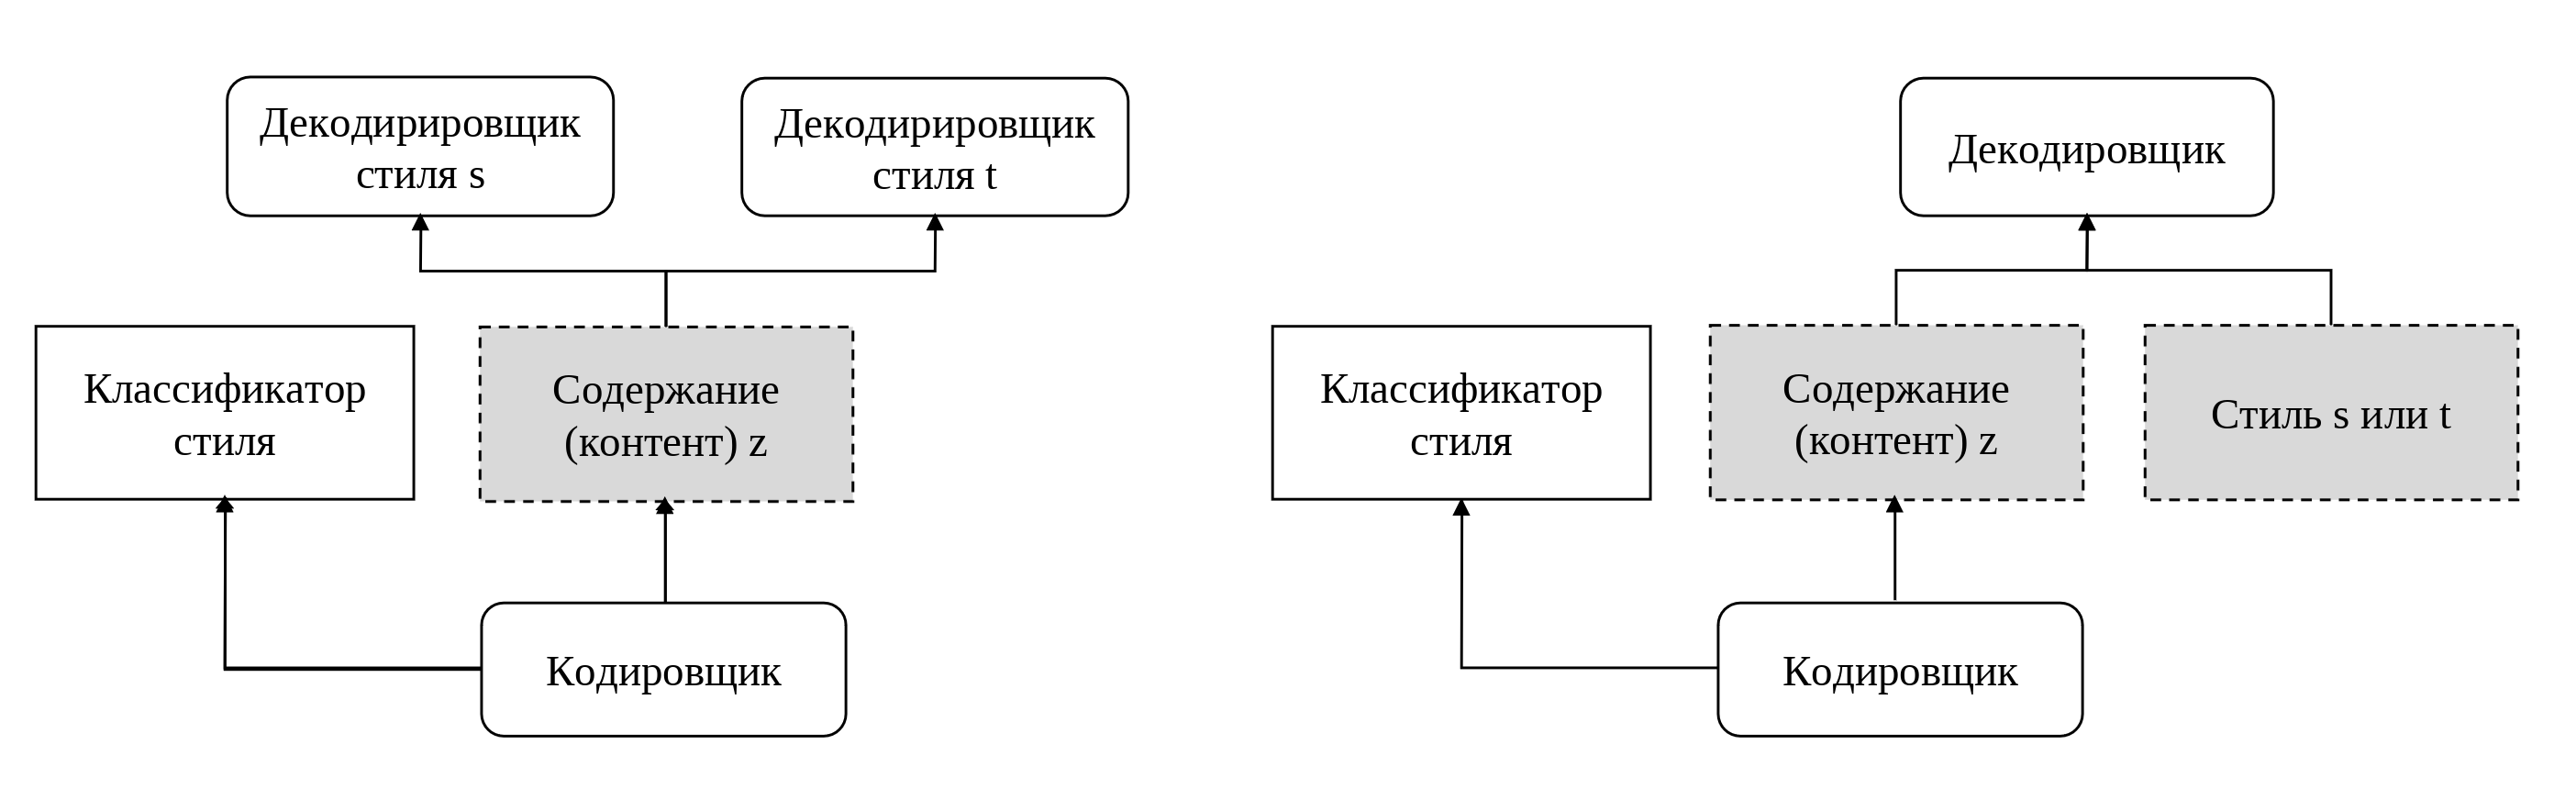
\includegraphics[width=1.0\textwidth]{figures/analysis_adversarial.png}}
  \caption{Состазательное обучение. Слева: подход с использованием нескольких декодировщиков. Справа: подход и использованием стилистических эмбеддингов}
  \label{fig:analysis_adversarial}
\end{figure}

Сама состязательная сесть состоит из двух главных компонент.
Первый компонент (дискриминатор) предназначен для классификации стиля входной последовательности $x$ на основе его латентного представления, созданного кодировщиком.
Функция потерь, которую необходимо минимизировать, -- это отрицательная логарифмическая вероятность меток стилей в обучающих данных:
$$
L_{adv1}(\Theta_D) =
- \sum_{i=1}^{M} \log p (l_i | \text{Encoder}(x_i; \Theta_E); \Theta_D)
$$
где $\Theta_D$ и $\Theta_E$ это параметры дискриминатора и кодировщика соответственно.  $M$ обозначает размер обучающего набора данных, а $l_i$ обозначает метку стиля.

Второй компонент предназначен для обмана дискриминатора, чтобы тот не мог правильно идентифицировать стиль входной последовательности $x$.
В этом случае функция потерь представляет собой максимизацию энтропии предсказаных меток стиля:
$$
L_{adv2}(\Theta_E) =
- \sum_{i=1}^M \sum_{j=1}^N
H(p(j|\text{Encoder}(x_i; \Theta_E); \Theta_D))
$$
где $N$ - количество стилей.
Обе части состязательной сети обновляют различный набор параметров.
Они работают вместе, чтобы гарантировать, что выход $\text{Encoder}(x_i;\Theta_E)$ не содержит стилистическую информацию.

Как только кодировщик обучен создавать латентное представление, два генеративных подхода генерируют текст в целевом стиле.
Первый подход подразумевает обучение нескольких декодеров под каждый стиль.
Второй подход использует обучение стилистических эмбеддингов и конкатенации их с представлением содержимого для генерации текста в целевом стиле с помощью декодера.

\subsection{Построение параллельного псевдо-корпуса}
\label{cha:analysis:subsection:backtranslation}
Обратный перевод (Back-Translation) изначально использовался в задаче машинного перевода для создания искуственного обучающего корпуса \cite{sennrich2016improving}.
Затем данный подход был успешно использован в задачах переноса стиля.
Выделяют два основных способа, основанных на поиске и генерации данных.

Первым из способов построения псевдопараллельных данных является поиск, а именно извлечение выровненных пар предложений из двух непараллельных корпусов в разных стилях.
В \textit{Unsupervised text attribute transfer via iterative matching and translation} \cite{jin2020imat} эмпирически показано, что семантически сходные предложения в двух стилистически разных корпусах, как правило, являются аналогами друг друга, отличающимися атрибутами стиля.
Следовательно, в работе строят изначальный псевдо-корпус путем сопоставления пар предложений в соответствии с косинусным сходством предварительно обученных эмбеддингов предложений.
Для каждого предложения $x$, его псевдо-аналог $\widehat{x'}$ это самое похожее предложение в другом корпусе $X'$:
$$
\widehat{x'} = \arg \max_{x' \in X'} \text{Similarity}(x, x')
$$

Второй способ является генеративным, такой как итеративный обратный перевод (Iterative Back-Translation, IBT) в работе \textit{Iterative back-translation for neural machine translation} \cite{hoang-etal-2018-iterative}.
Прежде чем начать итеративный процесс IBT должен инициализировать две модели преноса стиля: $M_{a \rightarrow a'}$, переводящая из стиля $a$ в стиль $a'$, и $M_{a' \rightarrow a}$, делающая обратное.
Затем на каждой итерации выполняется следующая последовательность шагов:
\begin{enumerate}
    \item Используются имеющиеся модели для генерации псевдо-параллельного корпуса.
    $M_{a \rightarrow a'}(x)$ генерирует псведо-пары $(x, \widehat{x'})$ для $\forall x \in X$,
    а $M_{a' \rightarrow a}(x)$ генерирует $(\widehat{x}, x')$ для $\forall x' \in X'$;
    \item Повторно обучаются эти две модели переноса стиля на наборах данных, сгенерированных на первом шаге.
    То есть обучаются $M_{a \rightarrow a'}(x)$ на парах $(\widehat{x}, x')$,
    а $M_{a' \rightarrow a}(x)$ на $(x, \widehat{x'})$.
\end{enumerate}

% На самом первом шаге простым вариантом инициализации является случайная инициализация двух моделей $M_{a \rightarrow a'}$ и $M_{a' \rightarrow a}$.
% Однако, так как этот способ подвержен случайности, обучение модели может не сойтись.




\subsection{Генерация с помощью управления атрибутами}
Этот метод подразумевает использование кода атрибута $a$ для управления генерацией текста в различных стилях.
% Существуют две стратегии генерации c помощью управления атрибутами:
% \begin{enumerate}
%     \item неявное ограничение латентного пространства $z$, чтобы оно содержало только информацию о содержимом, при изучении кода атрибута стиля;
%     \item без ограничения латентного пространства $z$ на содержание только информации о содержимом, при изучении кода атрибута стиля.
% \end{enumerate}

% В обоих стратегиях 
Функция потерь, управляемая классификатором, используется для гарантии того, что генератор $G$ сгенерирует предложение $x'$ с требуемым
атрибутом стиля.
А именно, функция потерь минимизирует:
$$
L_{cls}(\Theta_G, t) = -\mathbb{E}_{p(x)} [\log D(x')]
$$
где $D$ это классификатор стиля (дискриминатор), обученный на данных $x$.

Так как метод генерации с помощью управления атрибутами сильно зависит от классификатора стиля, этот подход имеет такие же недостатки, как и методы состязательного обучения.
В частности, точность классификатора стилей ограничивает выучивание качественных стилистических атрибутов.

В работе \textit{Toward controlled generation of text} \cite{hu2018controlled} используется вариационный автокодировщик (variational auto-encoder, VAE) \cite{kingma2022autoencoding}, который выучивает латентное пространство $z$, и классификатор стиля, чтобы выучить векто стилистических атрибутов $a$.
% Работа \textit{Toward controlled generation of text} \cite{hu2018controlled} является ярким представителем первой стратегии (неявное ограничение латентого пространства) и проиллюстрирована на рисунке \ref{fig:analysis_controled_text_generation}.
% Предлагаемая модель использует вариационный автокодировщик (variational auto-encoder, VAE) \cite{kingma2022autoencoding}, который выучивает латентное пространство $z$, и классификатор стиля, чтобы выучить векто стилистических атрибутов $a$.
Для этого используется следующая функция потерь:
$$
L_{VAE}(\Theta_G, \Theta_E; x) = 
KL(q_E(z|x) || p(z))
- E_{q_E(z|x)q_D(a|x)} [\log p_G (x| z,a)]
$$
где $KL(\cdot||\cdot)$ это дивергенция Кульбака-Лейблера, $\Theta_E$ и $\Theta_G$ -- параметры энкодера и декодера соответственно.
Условный вероятностный кодировщик $E$, обозначаемый как $q_E(z|x)$, выводит латентное представление $z$ по заданному входному предложению $x$.
$q_D(a|x)$ -- это условное распределение, определенное классификатором $D$ для каждой структурированной переменной в $a$. 
Общая схема модели проиллюстрирована на рисунке \ref{fig:analysis_controled_text_generation}.

Чтобы гарантировать, что $z$ сохраняет только информацию о семантике, не зависящую от стиля, предлагается ограничение независимости, гарантирующее, что латентное представление $z$ входного предложения $x$ и переданное предложение стиля $x'$ остаются близкими друг к другу.
Добавленное ограничение независимости, по существу, гарантирует, что информация о содержимом отделена от входного текста и закодирована в латентном представлении $z$.

\begin{figure}[ht]
  \centering
  \frame{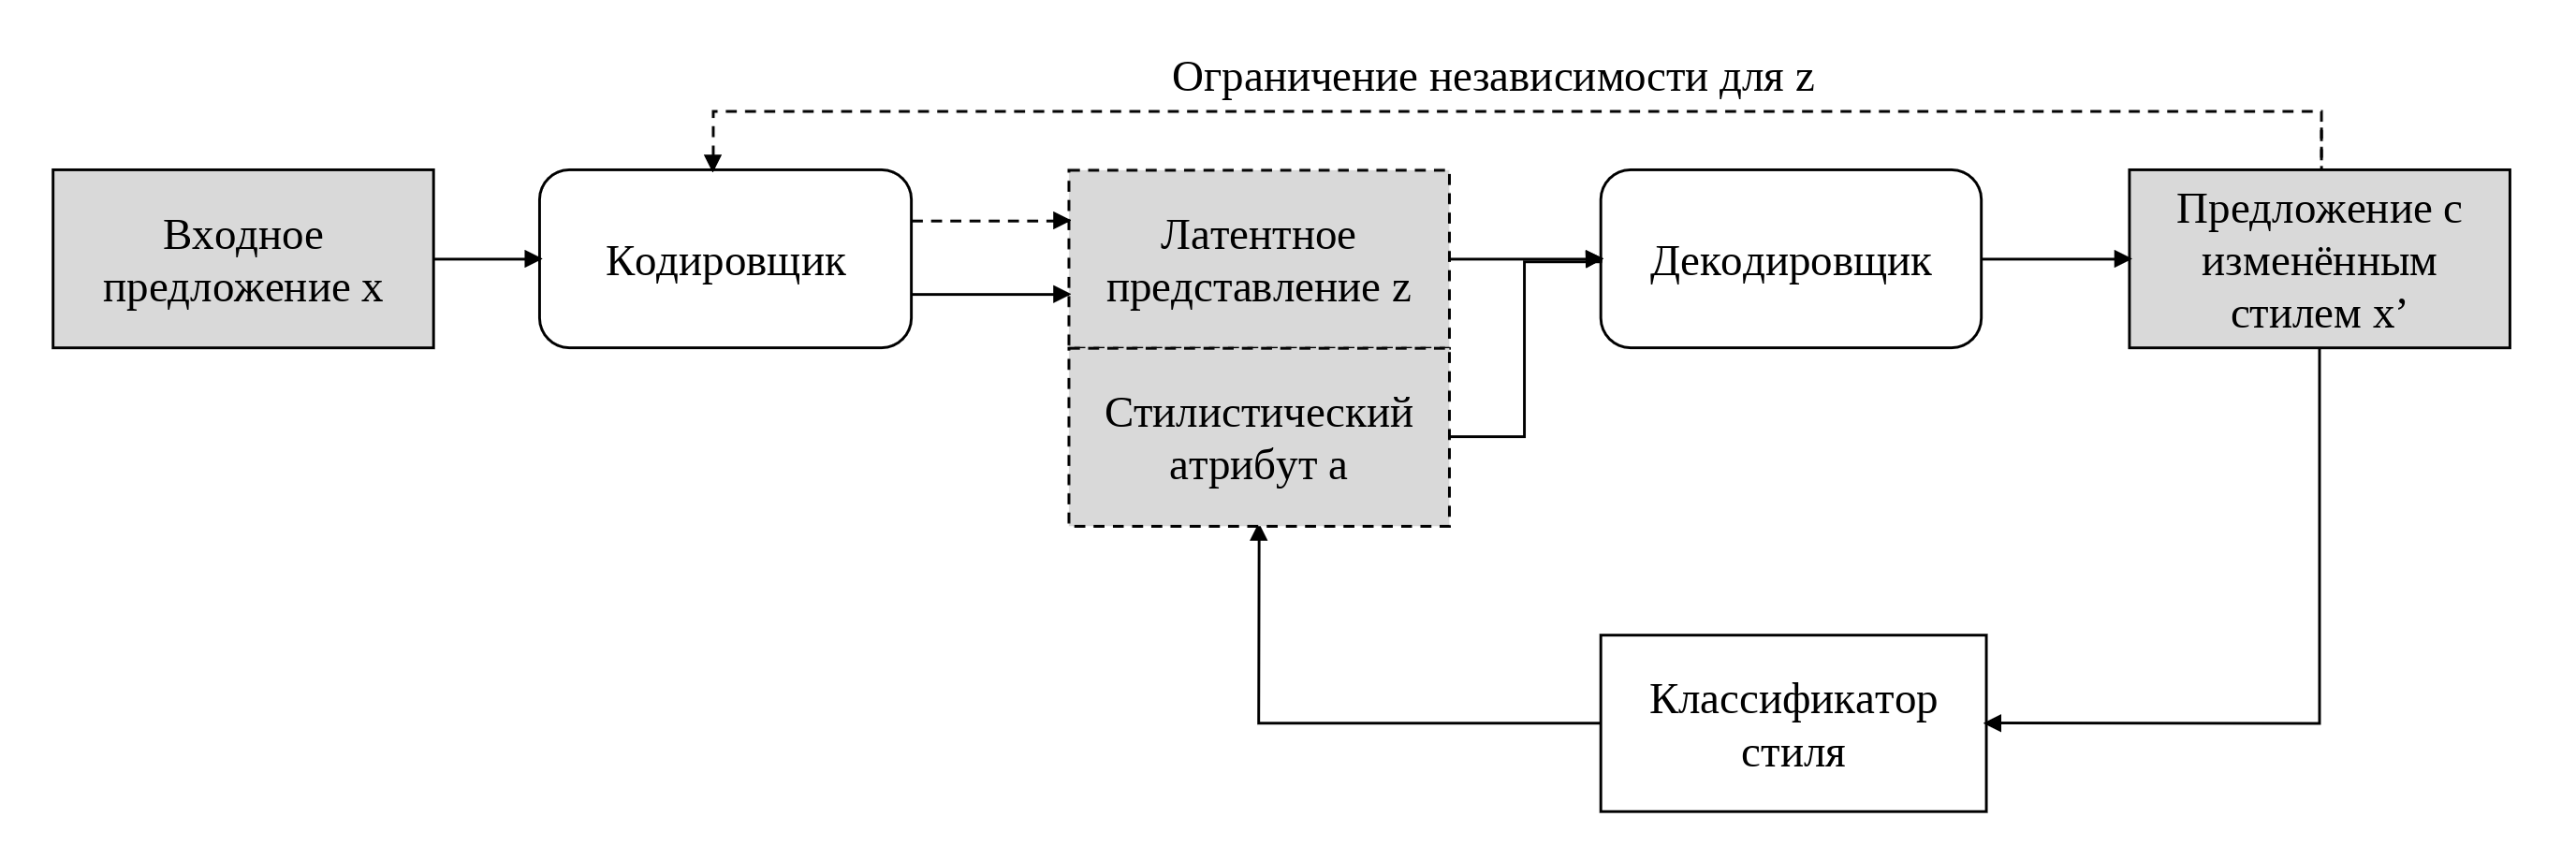
\includegraphics[width=1.0\textwidth]{figures/analysis_controled_text_generation.png}}
  \caption{Использование VAE для редактирования латентного пространства для трансфера стиля текста}
  \label{fig:analysis_controled_text_generation}
\end{figure}

% В работе \textit{Multiple-attribute text rewriting} \cite{subramanian2019multipleattribute} утверждалось, что задача разделения содержания и стиля в тексте является сложной.
% Поэтому, были предложены методы без этого.
% На рисунке \ref{fig:analysis_lample} проиллюстрированна модель, предложенная в этой работе.
% Модель использует варационный автокодировщик и механизм back-translation \ref{cha:analysis:subsection:backtranslation}.
% Сначала функция зашумления 

% \begin{figure}[ht]
%   \centering
%   \frame{\includegraphics[width=1.0\textwidth]{figures/analysis_lample.png}}
%   \caption{Генерация с помощью управления атрибутами с back-translation}
%   \label{fig:analysis_lample}
% \end{figure}

% ================================================================================
\subsection{Манипуляции в латентном пространстве}
Другим подходом к решению задачи переноса стиля текста является внесение изменений в латентное пространство, полученное от обучения модели автокодировщика.
%QUESTION: нужен тут риснок?
Рисунок \ref{fig:analysis_latent_repr_editing} иллюстрирует этот метод.
\begin{figure}[ht]
  \centering
  \frame{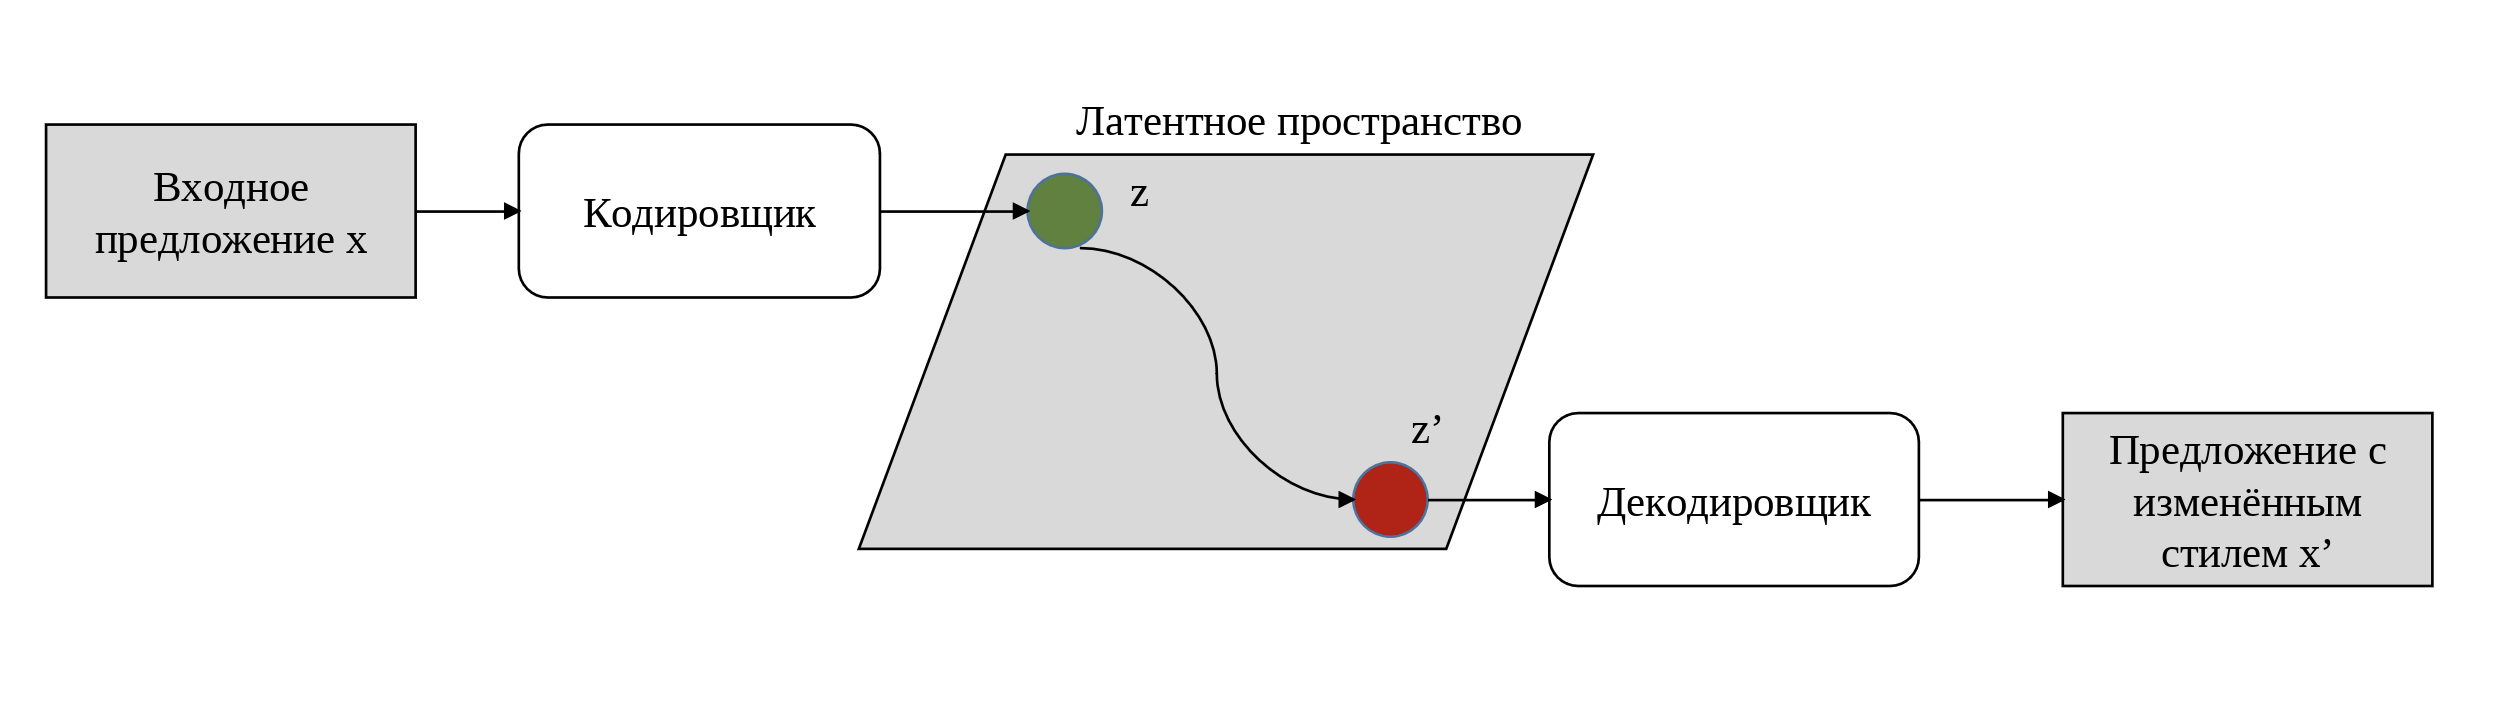
\includegraphics[width=1.0\textwidth]{figures/analysis_latent_repr_editing.png}}
  \caption{Общая структура редактирования латентного пространства для трансфера стиля текста}
  \label{fig:analysis_latent_repr_editing}
\end{figure}

% QUESTION автоэнкодер можно сказать?
Классификатор стиля обучается совместно с автоэнкодером.
Во время обучения итеративно обновляется латентное пространство $z$ в ограниченном пространстве, чтобы максимизировать точность классификатора.
А именно, каждое обновление вычисляется на основе градиента потери классификатора стилей относительно $z$.
Обработанное латентное представление $z'$ затем подаётся в декодер для генерации текста целевого стиля.

Главной проблемой методов этого семейства является определение границ, в пределах которых должна происходить манипуляция в латентном пространстве.
Было замечено, что декодер не может генерировать предложения в целевом стиле, если полученное после редактирования латентного пространства выходит за пределы областей представления, увиденных декодером во время обучения \cite{mueller_seq2betterseq}.
Существующие решения направлены на ограничение манипуляций в рамках ограниченного латентного пространства.


% ================================================================================
\subsection{Обучение с подкреплением}
Ключевая идея алгоритмов, основанных на обучении с подкреплением, это использование специально разработанных функций вознаграждения для управления процессом переноса стиля вместо различных функций потерь, используемых в
другим методах.

Алгоритм \textit{Policy Gradient} \cite{Williams1992SimpleSG} используется для максимизации ожидаемого вознаграждения за перефразированный текст.
% Алгоритм Policy Gradient упрощает обучение, не беспокоясь о сложности дискретного обучения, вызванной процессом автоматического регрессионного декодирования.
Однако из-за высокой дисперсии градиента выборки обучение с помощью этого метода может быть нестабильным.

В работе \textit{A Dual Reinforcement Learning Framework for Unsupervised Text Style Transfer} \cite{luo2019dual} предложено обучать две Seq2Seq модели между двумя стилями посредством обучения с подкреплением, не разделяя стиль и семантику.
Авторы рассматривали обучение модели переноса стиля из исходного в целевой и из целевого в обратный как двойную задачу.
Награда за классификатор стилей $R_S$ и награда за реконструкцию $R_C$ предназначены для повышения точности передачи стиля и сохранения семантики.
Общая награда является гармоническим средним из двух вознаграждений, и она использовалась в качестве сигнала обратной связи для обучения в
структуре с двумя задачами.
Таким образом, модель может быть обучена с помощью обучения с подкреплением без параллельных данных. Общая схема обучения представлена на рисунке \ref{fig:analysis_rl}
% QUESTION по термину "двойной" не уверен
% QUESTION нужна тут вообще картинка?
\begin{figure}[ht]
  \centering
  \frame{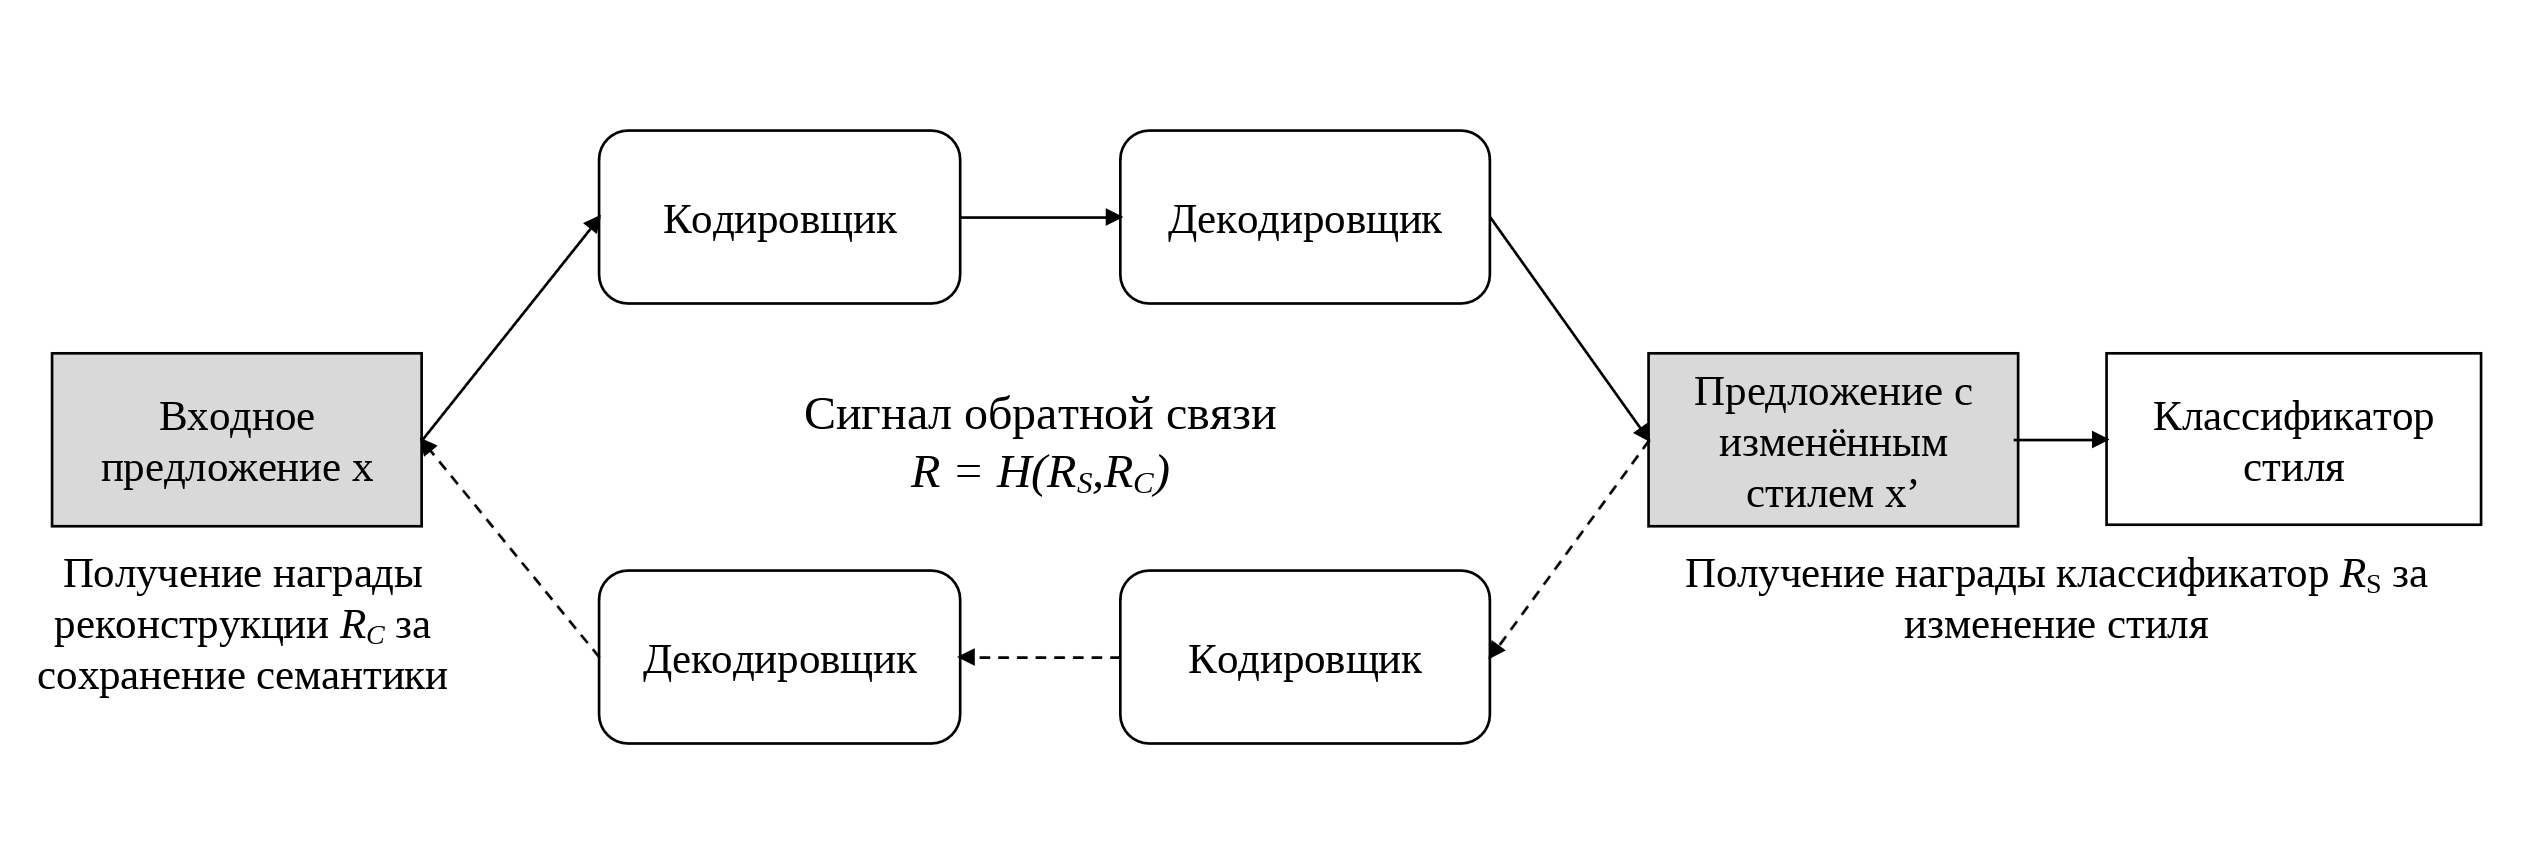
\includegraphics[width=1.0\textwidth]{figures/analysis_rl.png}}
  \caption{Модель двойного обучения с подкреплением}
  \label{fig:analysis_rl}
\end{figure}

Хотя существующие методы обучения с подкреплением по-прежнему в значительной степени опираются на классификаторы стилей для управления процессом переноса стиля, этот подход дает возможность разработать другие функции вознаграждения, которые будут направлять процесс переноса стиля.


\chapter{Создание набора данных} \label{cha:dataset}

На русском языке не существует набора данных, подходящего для целей исследования. 
Поэтому придётся создавать его самостоятельно.
Для этого потребуется определить два корпуса: первый, состоящий из текстов в формальном стиле, и второй, состоящий из текстов в неформальном стиле.
Затем, согласно главам \ref{cha:analysis:sec:target} и \ref{cha:analysis:sec:datasets}, для части предложений из неформального корпуса необходимо создать их формальные парафразы.

\section{Обзор наборов данных, подходящих для аннотации}
Можно определить доступные корпуса на русском языке: Википедия, новостные издания, литература, печатные издания, субтитры, социальные сети, специализированные наборы данных для конкретных задач (например, детоксификация текста).

Социальные сети на первый взгляд подходят для создания неформального корпуса, однако стилистические атрибуты в них крайне неоднородны и значительно различаются у разных пользователей. Так же большое количество пользователей использует достаточно нейтральный стиль в своих комментариях.

% Луркморе как антипод википедии. Стилестически выдержаный. Достаточный объём.
Интересным кандидатом для использования в качестве источника неформального текста является база статей сайта Луркморье\footnote{Оригинальный сайт удалён владельцем. Обновлённая версия: https://neolurk.org/wiki/Луркморье} (Lurkmore) за 2021 год.
Луркморье -- русскоязычная интернет-энциклопедия, аналог Википедии, функционирующая на том же движке MediaWiki, но написанная в неформальном стиле, изобилующая жаргонами и интернет-мемами, и позиционирующая себя как <<энциклопедия современной культуры>>.
Данный сайт, помимо того, что удовлетворяет критерию неформального стиля, является стилистическим антиподом Википедии.
Также база статей имеет достаточный объём (около 9 тысяч статей, состоящих из более 600 тысяч предложений различной длины) для использования в обучении современных нейросетевых алгоритмов.

В данной работе выбор был сделан в пользу пары Луркморье-Википедия. Главной причиной такого решения является жанровая близость двух этих корпусов (здесь под жанром подразумевается функциональная направленность текста, как в работе \textit{Functional Text Dimensions for annotation of Web corpora} \cite{sharov_corpora}). Тексты из обоих корпусов являются энциклопедическими статьями, информирующими читателя о объектах действительности и явлениях. 

Для разбивки текста на предложения был использован токенизатор Razdel от проекта Natasha\footnote{https://github.com/natasha/razdel}.
Затем принимались только предложения, соответствующие следующим параметрам:
\begin{itemize}
    \item длина от 80 символов
    \item минимум 5 слов в предложении
    \item обязательно должна присутствовать кирилица.
\end{itemize}
Из базы можно получить около 423 тысяч предложений, что соответствует 125 МБ текста.
Таким образом в итоговом корпусе оказалось 423974 предложения.


\section{Разметка данных}
\subsection{Толока}
Как было упомянуто в \ref{cha:analysis:sec:target} 10000 пар предложений формальный-неформальный стиль являются желаемым результатом. Такое в одиночку не сделать, поэтому необходимо воспользоваться помощью асессоров. И подходящим сервисом для решения этой задачи является сервис Толока\footnote{https://toloka.ai/} -- платформа для привлечения асессоров к разметке данных.

% Однако, следует обратить внимание на наборы данных, изначально собранных для похожих задач, а также на других языках. Потому что это лучше поможет понять задачу и убережёт от вероятных ошибок в создании собственного набора данных.
Основная сложностью в процессе привлечения сторонних людей является описание задания, написание инструкции и фильтр подходящих кандидатов \cite{dementieva2021crowdsourcing}.

% Тестовый запуск на 100 предложений. Описание запуска. Результаты. Ошибки толокеров. Дороговизна
Для проверки работоспособности подхода было принято решение запустить тестовое задание на 100 случайных предложений из выборки.
На рисунках \ref{fig:toloka_instruction_1} и \ref{fig:toloka_instruction_2} представлена инструкция, выдаваемая асессорам. 
В ней пользователю Толоки объясняется, что нужно перефразировать предложения из сленга в формальный стиль.
Даётся пример источников текста в формальном стиле.
Затем приводится несколько примеров перефразов.
В инструкции также указывается предупреждение, что в задании может содержаться оскорбительный контент.
Также толокеру сообщается, что неформальность заключается не только в наличии сленга, но и в стилистике предложения. Приведены несколько примеров.
Указывается, что в случае невозможности перевести предложение или в случае, если толокер считает его уже формальным, необходимо его пропустить

\begin{figure}[ht]
  \centering
   \frame{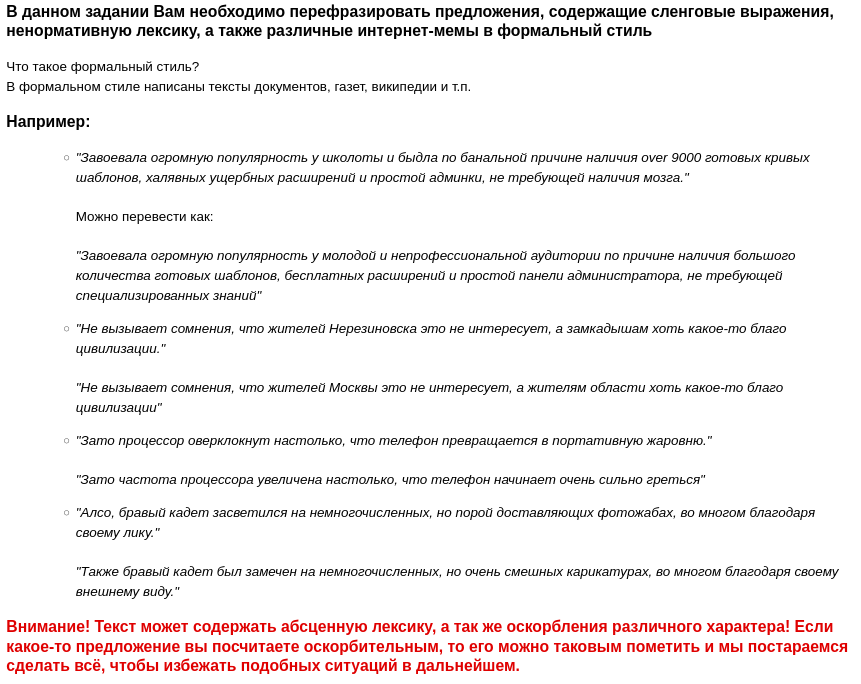
\includegraphics[width=\textwidth]{figures/toloka_instruction_1.png}}
  \caption{Первая часть инструкции для разметчиков}
  \label{fig:toloka_instruction_1}
\end{figure}

\begin{figure}[ht]
  \centering
  \frame{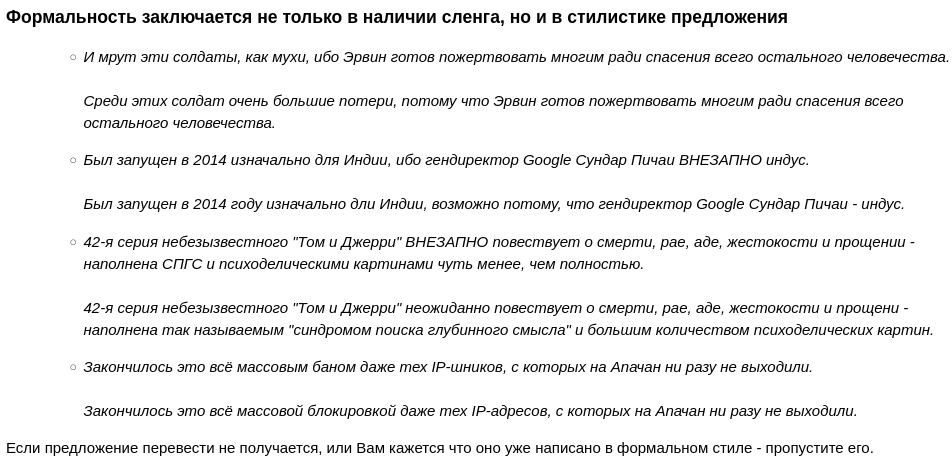
\includegraphics[width=\textwidth]{figures/toloka_instruction_2.png}}
  \caption{Вторая часть инструкции для разметчиков}
  \label{fig:toloka_instruction_2}
\end{figure}

Само задание представляет лишь обязательное поле, в которое асессор должен записать парафраз.
Изображение интерфейса задания представлено на рисунке \ref{fig:toloka_input_field}.
На одну страницу давалось одно задание, чтобы асессор мог на нём сфокусироваться. Временной лимит устанавливался в 10 минут.

\begin{figure}[ht]
  \centering
  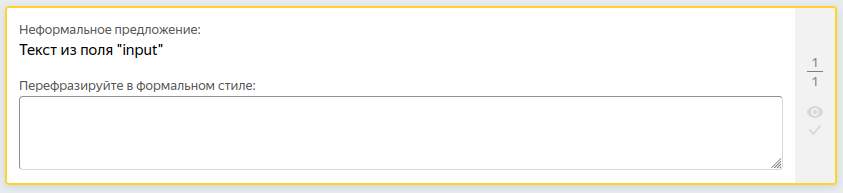
\includegraphics[width=\textwidth]{figures/toloka_input_field.png}
  \caption{Окно задания для разметчика}
  \label{fig:toloka_input_field}
\end{figure}

Так же было установлено тридцатипроцентное качество исполнителей. Установлено перекрытие равное 2, т.е. каждое предложение продублируется двум разным исполнителям.
И, самое главное, была установлена отложенная приёмка, что означает, что асессоры получат деньги, лишь при явном одобрении результата.
Полный список настроек представлен на рисунке \ref{fig:toloka_settings}.

\begin{figure}[ht]
  \centering
  \frame{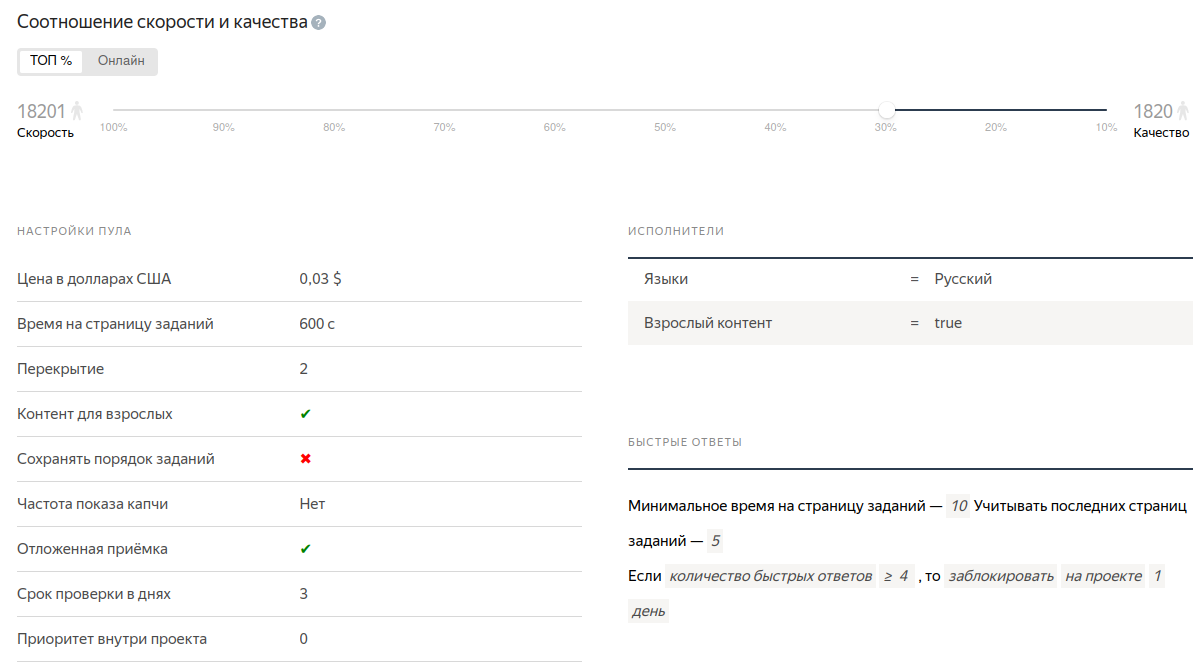
\includegraphics[width=\textwidth]{figures/toloka_settings.png}}
  \caption{Параметры задания}
  \label{fig:toloka_settings}
\end{figure}

Получились следующие результаты. Для 100 предложений с перекрытием 2 было создано 200 заданий. После ручной проверки были приняты 96 перефразов, 44 был отклонены и с 60 ответами возникли трудности. Постановку задачи можно считать удовлетворяющей.

Однако, у многих асессоров возникли некоторые трудности:
\begin{itemize}
    \item Грамматические ошибки. Исполнитель либо опечатался, либо использовал неправильно причастие или спряжение, таких случаев немного. Такие предложения можно принять, потому что эти ошибки можно легко выявить и исправить.

    \item Формализована лишь часть предложения. Распространённый случай, когда, например, исполнитель заменил обсценное слово на нейтральное, но в тоже время не затронул другие стилистически неформальные конструкции.

    \item Исполнитель не понял сленга. Здесь исполнитель либо не распознал отсылку на интернет-мем, либо неправильно её понял.

    \item Искажён смысл. Ошибка зачастую связанная с предыдущей, когда асесор очевидным образом изменил посыл предложения.

    \item Также распространены случаи, когда исполнитель вроде перефразировал, выполнил задачу, но стилистически текст всё ещё несёт в себе просторечия.
\end{itemize}

Сразу появилось много идей, как можно улучшить качество:
\begin{itemize}
    \item Добавить обучение
    \item Увеличить соотношение качество/скорость
    \item Увеличить перекрытие (затратно)
    \item Запускать разметку по частям и отфильтровывать исполнителей
    \item Расписать более подробно критерии приёмки
    \item Уменьшить длину предложений
\end{itemize}

Также необходимо оценить финансовые затраты.
В среднем асессор тратил около двух минут на выполнение задания (немного медленнее, чем в \cite{dementieva2021crowdsourcing}), соответственно он может выполнять 30 заданий в час.
Если установить цену в \$0,02 за задание, то один асессор обходится в \$0,6/час.
Тогда необходимые 10000 предложений обойдутся в \$200, что по курсу 80 рублей за доллар будет составлять 16000 рублей.
Данная цена является достаточно большой.

% На этом этапе было рекомендовано обратиться к студентам-лингвистам из РГГУ и попросить помочь их с разметкой данных. И спасибо Александре Ивойловой и её студентам, что откликнулись и начали помогать нам с данными.

\subsection{Привлечение студентов из РГГУ}
% Привлекли студентов р, спасибо Александре Ивойловой. Разработали программу для разметки. Поставили им цели/задачи, учли опыт яндекса. 4 месяца получали длилось. Результаты.

В связи с этими проблемами было рекомендовано обратиться к студентам-лингвистам из Российского Государственного Гуманитарного университета и попросить помочь их с разметкой данных. Спасибо Александре Ивойловой и её студентам, что откликнулись и начали помогать с выполнением работы.

В создании набора данных приняли участие 16 студентов старших курсов.
Им были объяснена специфика и проблемы, возникшие на Толоке.

Целью было поставлено собрать 10000 перефразированных предложений. Для оценки качества работы алгоритма этого будет достаточно.

Для выполнения задачи Александра Ивойлова и я создали небольшую программу, которая автоматически сохраняла результаты и различные метрики. Интерфейс программы представлен на рисунке \ref{fig:data_tool_rggu}.

\begin{figure}[ht]
  \centering
  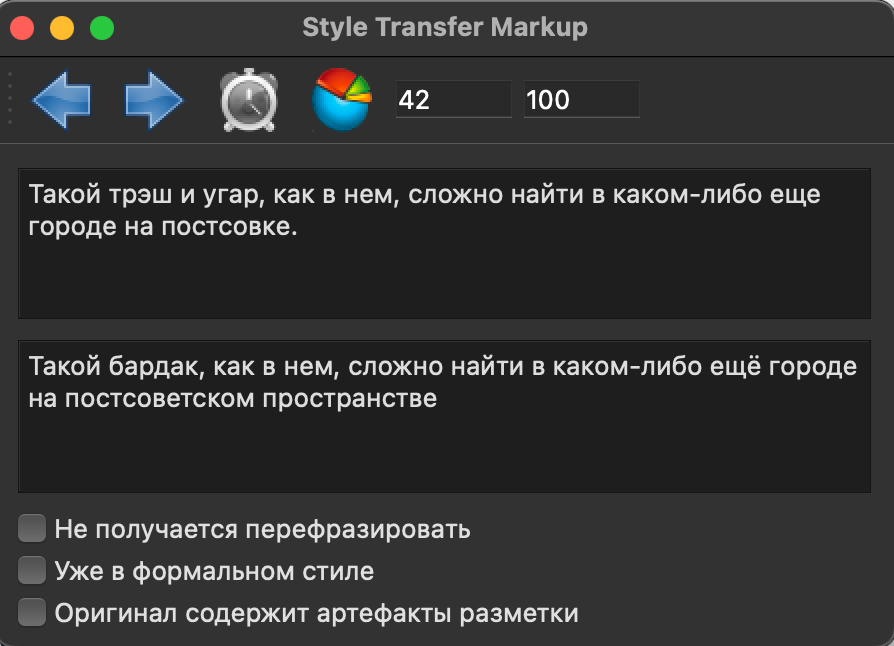
\includegraphics[width=0.8\textwidth]{figures/data_tool_rggu.png}
  \caption{Программа разметки данных для студентов РГГУ}
  \label{fig:data_tool_rggu}
\end{figure}

Вверху указано переводимое предложение, а в нижнем окне студент должен записать свой парафраз.
Так же, если предложение вызывает трудности у студента, то его можно соответствующим образом пометить.
Это сделано для того, чтобы можно было в дальнейшем фильтровать предложения.
Если оригинал содержит артефакты разметки, то можно его исправить после разметки и получить хорошее предложение. Артефакты разметки означают, что само исходное предложение качественное, но в нем остались артефакты от вики-движка и нужно вручную их почистить.


Аннотирование длилось четыре месяца и были получены следующие результаты:
\begin{itemize}
    \item Всего обработано 30118 предложений;
    \item 17881 предложение готовы к использованию;
    \item 1271 одно предложение были помечены как имеющие артефакты. После исправления артефактов и фильтрации осталось 659 предложений.
\end{itemize}
Итого получилось 18 540 предложений. Поставленная цель перевыполнена.

Студенты перевели большую часть неформальностей, интернет-мемов и отсылок, а те, которые они не понимали, искали им объяснения в интернете и пытались сделать хороший перевод.
В целом эту работу можно оценить как положительную.


Однако, некоторые аспекты можно было выполнить лучше.
Со стороны студентов: несмотря на просьбы пропускать очевидно формальные предложения, часто студенты их не игнорировали и переписывали с минимальными изменениями.
С нашей стороны необходимо было более качественно подходить к фильтрованию набора данных и инвестировать больше времени в поиск более качественного алгоритма по формированию выборки.

\chapter{Проведение экспериментов} \label{cha:experiments}
% QUESTION НУЖНО ЛИ ПЕРЕРИСОВЫВАТЬ КАРТИНКИ? А ССЫЛКИ НА КАРТИНКИ?

\section{Используемые инструменты}
% QUESTION: нужно это вообще?
Разработка велась на языке программирования \textit{Python 3.8}.
% QUESTION: правильно сослался?
Реализация нейронных сетей и оценка качества выполнены с помощью библиотек \textit{PyTorch} \cite{pytorch_lib}, \textit{transformers} и \textit{evaluate} от проекта \textit{HuggingFace} \cite{huggingface_transformers}.
Предобученные модели получены из \textit{HuggingFaceHub}, открытого репозиторя моделей и наборов данных.
Обучение выполнялось на видеокарте Nvidia T4.

\section{Метрики качества}
% QUESTION: тут цитаты нужно сделать? а что конкретно за веса, что взяты из хаггингфейса нужно сказать? если да, то как? а на берт нужно сослаться?

Для оценки качества алгоритма будут использоваться следующие метрики:
\begin{itemize}
    \item SacreBLEU \cite{sacrebleu};
    \item METEOR \cite{meteor};
    \item 
    Style Score -- дообученный с помощью параметро-эффективного метода LoRA \cite{lora} на собранном наборе данных классификатор стиля.
    В качестве изначальных весов взят \texttt{xlm-roberta-base}. Качество классификатора:
    \texttt{Accuracy}: 86\%,
    \texttt{F-1}: 86\%,
    \texttt{Precision}: 91\%,
    \texttt{Recall}: 83\%;
    \item 
    Semantic Score -- дообученный с помощью параметро-эффективного метода LoRA \cite{lora} на собранном наборе данных классификатор семантики, определяющий как сильно сохраняют два предложения одно и то же содержание.
    В качестве изначальных весов взят \texttt{cointegrated/rubert-tiny2}. Качество классификатора: 
    \texttt{Accuracy}: 85\%,
    \texttt{F-1}: 86\%,
    \texttt{Precision}: 91\%,
    \texttt{Recall}: 82\%.
\end{itemize}

\section{Обучение без учителя: Denoising Auto-Encoder}
% TODO подводку побольше
% QUESTION Этого одного цитирования достаточно на всё?
Генерация с помощью управления атрибутами с использованием архитектуры denoising auto-encoder \cite{lample2018unsupervised, lample2018phrasebased, subramanian2019multipleattribute} является распространённым решением в ситуации отсутствия параллельных данных.
% Естественным решением в ситуации отсутствия параллельных данных является unsupervised подход, который представлен denoising auto-encoder’ом \cite{lample2018unsupervised, lample2018phrasebased, subramanian2019multipleattribute}.

% Основная идея и принципы
% \subsection{Принципы}
% Задача изменения формальности текста является плохо сформулированной задачей, потому что потенциально существует множество способов перефразировать исходное предложение, особенно в неформальный стиль. 
% Тем не менее за последние годы был достигнут впечатляющий прогресс в достижении этой цели и были выделены основные принципы обучения без учителя, как для задачи переноса стиля текста, так и для задачи машинного перевода.

В данном подходе были выработаны три принципа для решения задачи.
Визуализация этих принципов представлена на рисунке \ref{fig:lample_principles}.
На изображении под пунктом A показаны исходные данные: два набора данных, каждый со своим стилем (разные цвета и точки соответствуют предложениям с соответствующим стилем).
Под пунктом Б представлен первый принцип: инициализация. Делается так, чтобы оба распределения примерно совпадали, например, с помощью дословного перевода с использованием словаря.
В пункте В проиллюстрирован второй принцип: языковое моделирование. Языковая модель обучается независимо для каждого стиля для определения структуры данных (изображено в виде непрерывной кривой); она действует как основанная на данных система для устранения шума / исправления предложений (проиллюстрировано пружиной, втягивающей предложение за пределы многообразия обратно).
И, наконец, под пунктом Г изображен третий принцип: обратный перевод (см. \ref{cha:analysis:subsection:backtranslation}).
Начиная с наблюдаемого исходного предложения (заполненный красный круг), используется текущая модель для парафраза (пунктирная стрелка), что приводит к потенциально неправильному переносу стиля (синий крестик рядом с пустым кругом).
Начиная с этого (обратного) перевода, используется модель для переноса стиля в обратную сторону (непрерывная стрелка) для восстановления предложения в оригинальном стиле.
Несоответствие между восстановлением и исходным предложением является сигналом ошибки для обучения параметрам модели.
    Та же процедура применяется в обратном направлении.
\begin{figure}[ht]
  \centering
  \frame{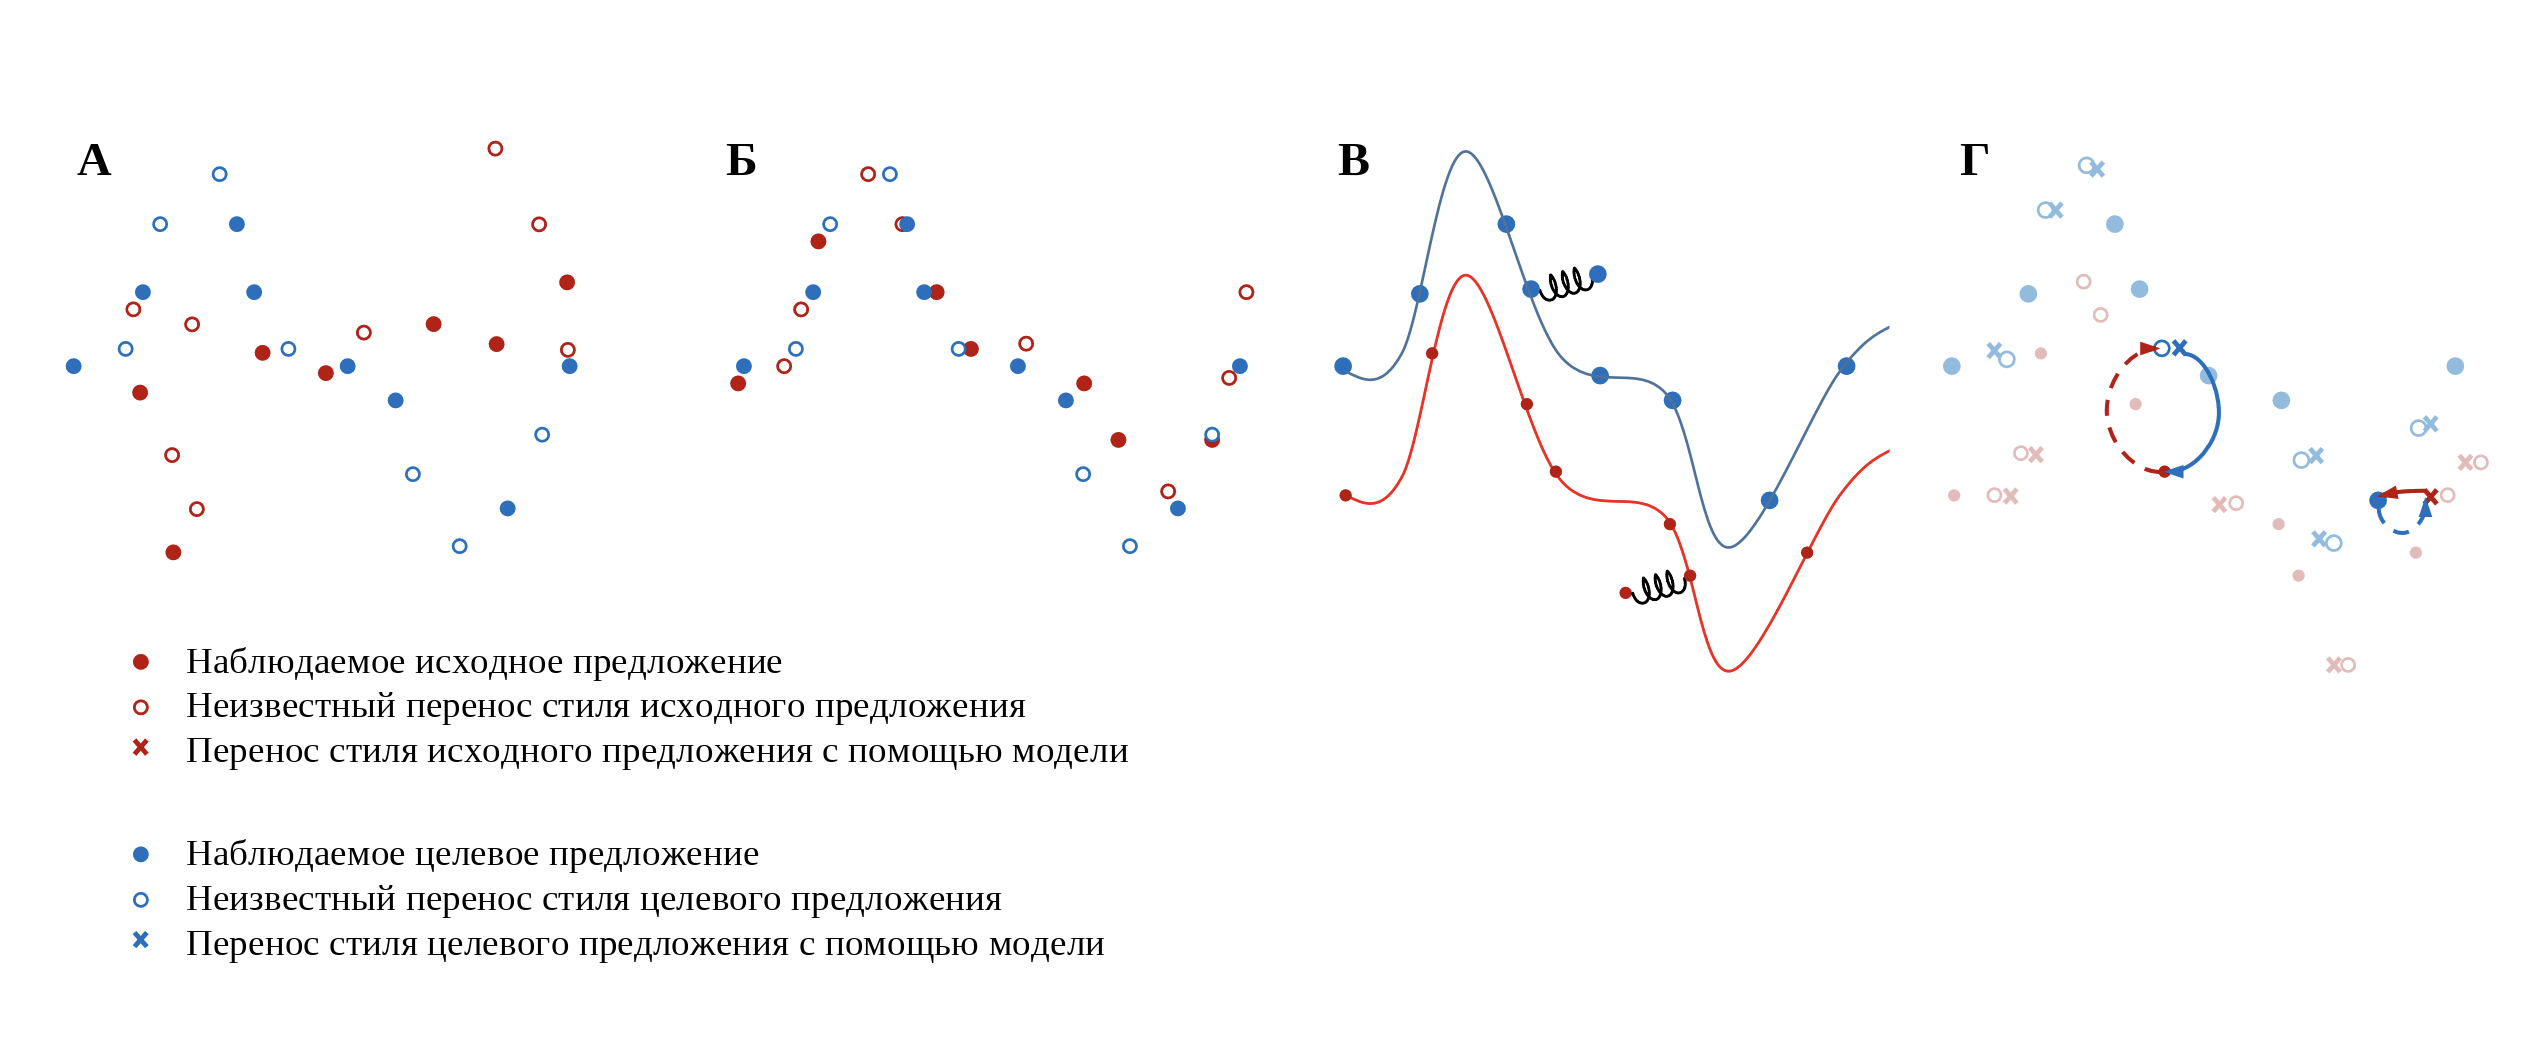
\includegraphics[width=\textwidth]{figures/lample_principles.png}}
  \caption{Принципы алгоритмов "без учителя" для задачи переноса стиля текста}
  \label{fig:lample_principles}
\end{figure}

% Архитектура (в разрезе принципов)
% \subsection{Архитектура модели}
% TODO: overview?
% QUESTION: алгоритм может в виде листинга представить??
% QUESTION: обозначиМ можно? можно в первом лице?
% Листинг алгоритма приведён на рисунке \ref{fig:lample_algorithm}.
% \begin{figure}[ht]
%   \centering
%   \frame{\includegraphics[width=\textwidth]{figures/lample_algorithm.png}}
%   \caption{Алгоритм обучения без учителя для переноса стиля текста}
%   \label{fig:lample_algorithm}
% \end{figure}

% \begin{figure}[ht]
%   \centering
%   \frame{\includegraphics[width=1.0\textwidth]{figures/analysis_lample.png}}
%   \caption{Генерация с помощью управления атрибутами с back-translation}
%   \label{fig:analysis_lample}
% \end{figure}

На этапе инициализации, вместо рассмотрения отдельных слов в предложении, используются byte-pair encoding токены (BPE-токены) \cite{bpe_tokens_article}.
Подобная токенизация даёт два больших преимущества: уменьшает размер словаря и избавляет от присутствия неизвестных UNK-токенов в перефразированном предложении.
BPE-токены обучаются на совместном наборе данных обоих стилей, так как язык одинаковый и большая часть этих токенов будет совпадать. Помимо прочего, в таком случае отпадает необходимость получать словарь между словами разного стиля.
Затем, обучаются word2vec эмбеддинги токенов \cite{mikolov2013distributed}, который затем будут использованы в языковой модели.

% Языковая модель состоит из 
Этап языкового моделирования представлен автокодировщиком с шумоподавлением (denoising autoencoder, DAE) \cite{dae_article, lample2018phrasebased}.
Архитектурой автокодировщика является transformer \cite{attention_is_all_you_need}.
Без каких-либо ограничений обычный автокодировщик очень быстро учится просто копировать каждое вводимое слово одно за другим.
Такая модель также идеально копировала бы последовательности случайных слов, предполагая, что модель не выучивает какую-либо полезную структуру в данных.
Чтобы решить эту проблему, во входные предложения добавляется шум \cite{hill2016learning} и применяется стратегия подавления шума, получая Denoising Autoencoder -- автокодировщик с шумоподавлением \cite{dae_article}.
Общая схема представлена на рисунке \ref{fig:lample_dae}, а функция потерь задаётся как:
$$
\mathcal{L}^{lm} = 
\mathbb{E}_{x \sim \mathcal{S}} [-\log P_{s \rightarrow s}(x|C(x))] +
\mathbb{E}_{y \sim \mathcal{T}} [-\log P_{t \rightarrow t}(y|C(y))]
$$

где $C$ - функция зашумления, которая удаляет или меняет местами некоторые слова \cite{lample2018unsupervised}, а $P_{s \rightarrow s}$ и $P_{t \rightarrow t}$ - композиции энкодера и декодера, оперирующие в исходном или целевом пространстве соответственно.

% QUESTION рассказать подробнее про функцию зашумления?

\begin{figure}[ht]
  \centering
  \frame{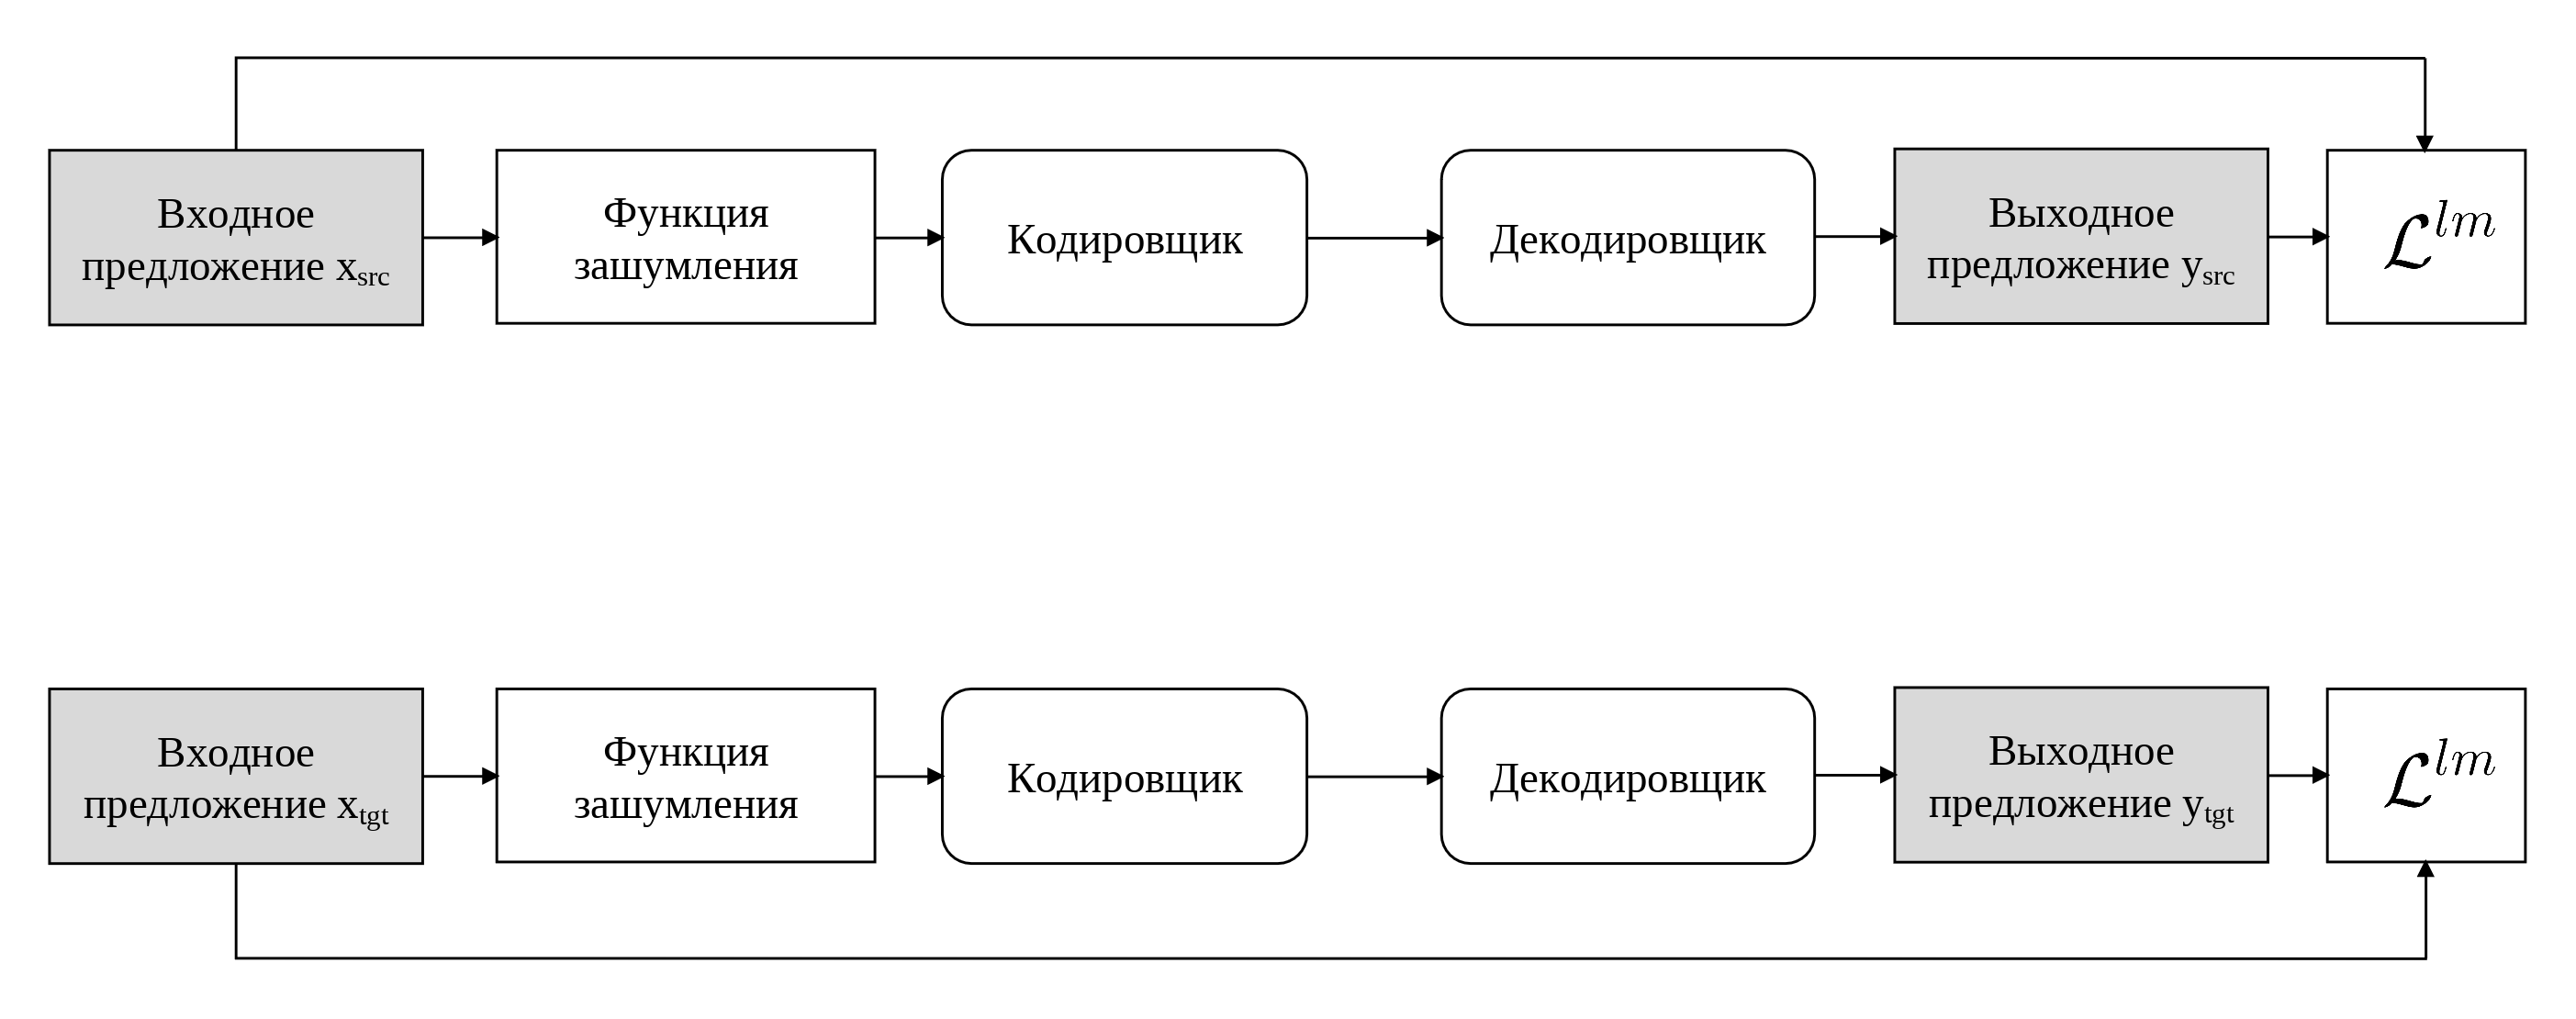
\includegraphics[width=\textwidth]{figures/lample_dae.png}}
  \caption{Обучение denoising auto-encoder}
  \label{fig:lample_dae}
\end{figure}

% Итеративный обратный перевод

% На этом основан механимз back-translation: применим имеющуюся на данную итерацию модель для перевода стиля. Получим парафраз определенного качества. И на полученный парафраз применим обратный перевод: зашумим и пропустим обратно через модель в надежде, что мы сможем восстановить изначальное предложение.

Пространство предложений в исходном и целевом стиле обозначается через $\mathcal{S}$ и $\mathcal{T}$ соответственно, а языковые модели, обученные на исходных и целевых наборах данных, через $P_s$ и $P_t$, соответственно.
Через $P_{s \rightarrow t}$ и $P_{t \rightarrow s}$ обозначим модели парафраза из исходного стиля в целевой и наоборот.
Пусть $u^*(y)$ это предложение в исходном стиле, полученное из $y \in \mathcal{T}$ такое, что $y^*(y) = \arg\max P_{t \rightarrow s}(u|y)$. Подобным образом пусть $v^*(x) = \arg \max P_{s \rightarrow t}(v|x)$.
Таким образом пара $((u^*(y), y)$ и $(x, v^*(x)))$ представляет автоматически перефразированные параллельные предложения, которые могут быть использованы для обучения модели, минимизируя следующую функцию потерь:
$$
\mathcal{L}^{back} = 
\mathbb{E}_{y \sim \mathcal{T}} [-\log P_{s \rightarrow t}(y|u^*(y))] +
\mathbb{E}_{x \sim \mathcal{S}} [-\log P_{t \rightarrow s}(x|v^*(x))]
$$
Этим и выражается третий принцип. Общая схема представленна на рисунке \ref{fig:lample_backtranslation}.

\begin{figure}[ht]
  \centering
  \frame{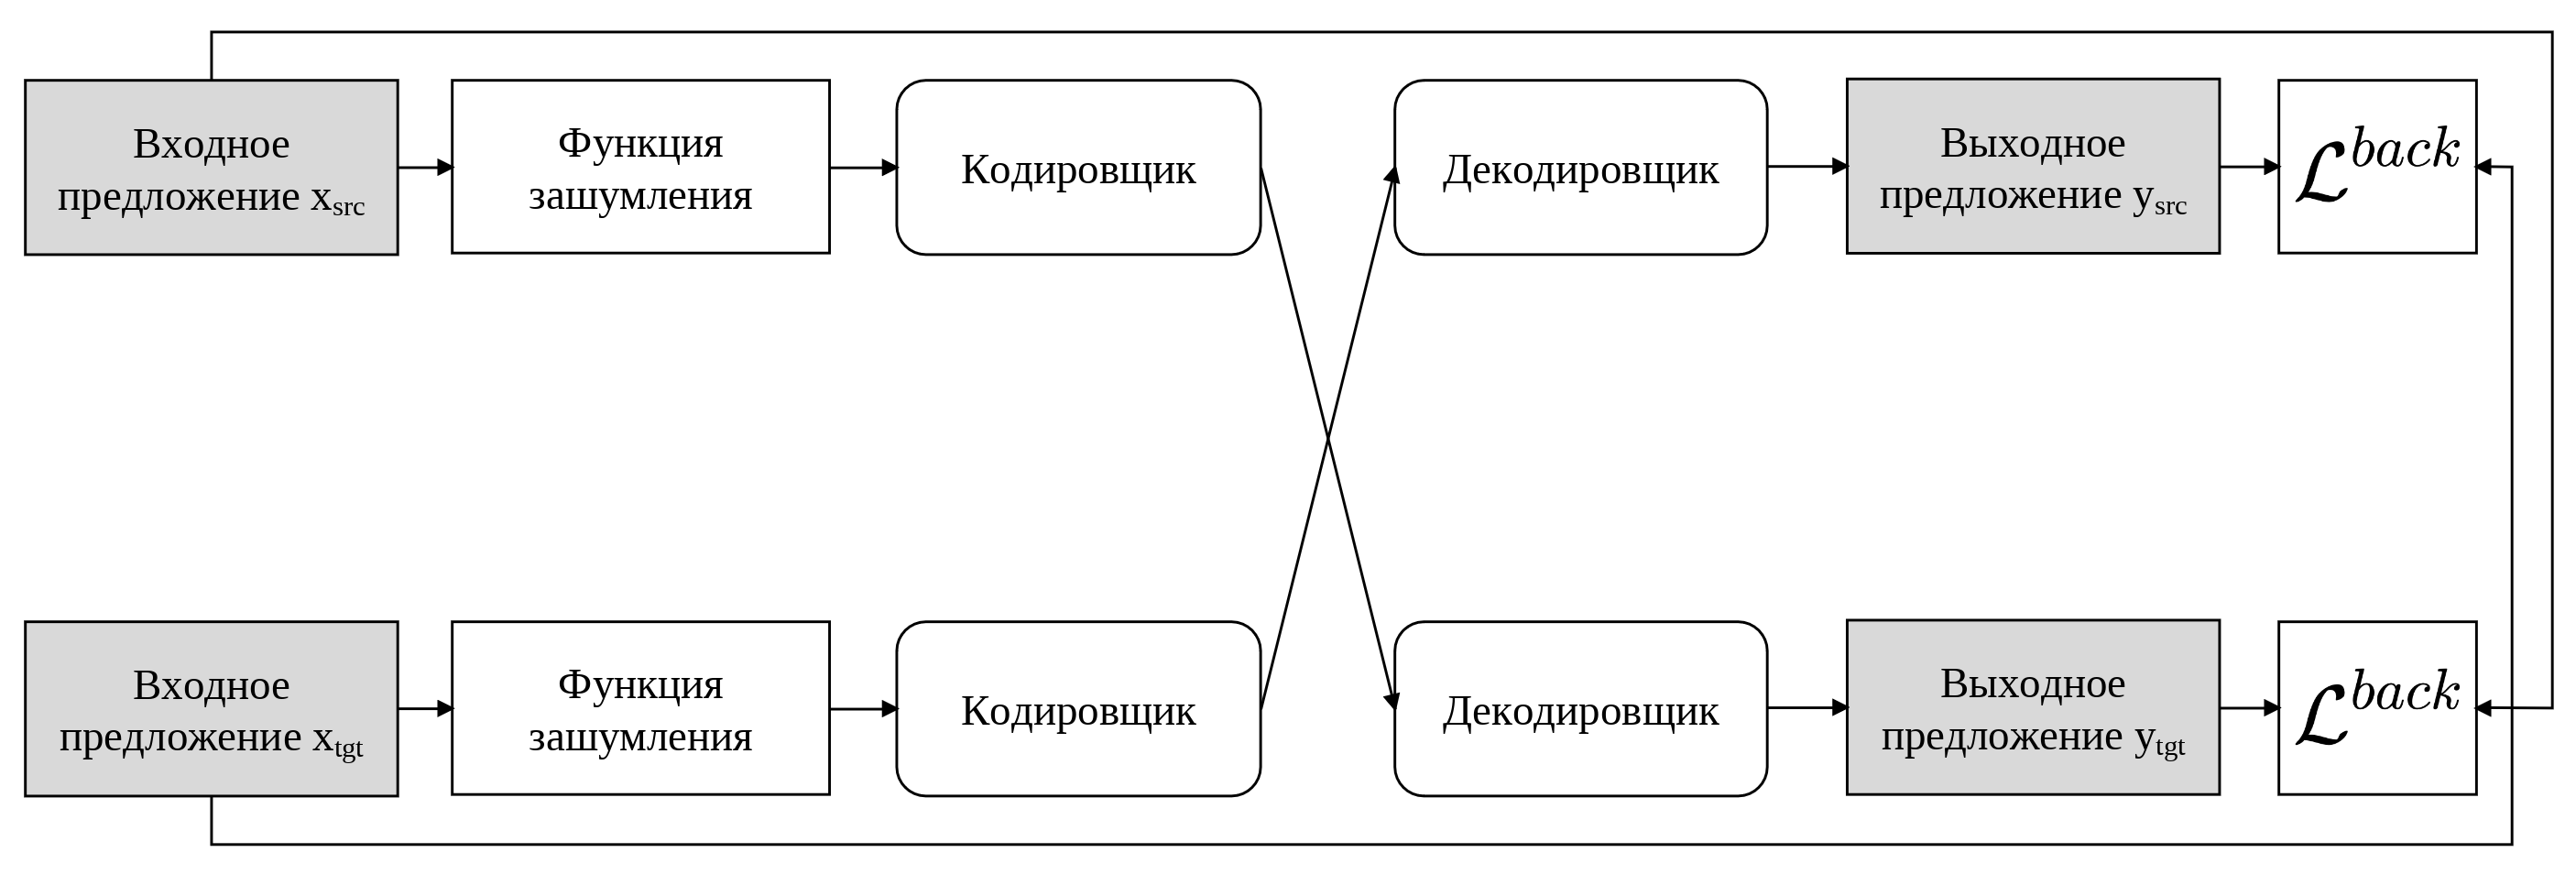
\includegraphics[width=\textwidth]{figures/lample_backtranslation.png}}
  \caption{Обучение с помощью back-translation}
  \label{fig:lample_backtranslation}
\end{figure}

% Он задается 3-мя целевыми функциями:
% \begin{enumerate}
%     \item Это сам авктокодировщик: как хорошо модель может восстановить зашумлённое предложение. Ключевой фактор это функция зашумления, без неё модель будет просто копировать предложения. Здесь эта функция случайным образом удаляла и переставляла местами слова.
%     \item Это функция потерь дискриминатора: дополнительно обучается дискриминатор, который классифицирует исходный стиль эмбеддинга в латентном пространстве. Этот адверсариал-лосс может показаться важным, но на самом деле дальнейшие исследования и мой опыт обучения показывают, что он играет минимальную роль
%     \item И, наконец, третье – самое главное – это кросс-доменная функция потерь. На этом основан механимз back-translation: применим имеющуюся на данную итерацию модель для перевода стиля. Получим парафраз определенного качества. И на полученный парафраз применим обратный перевод: зашумим и пропустим обратно через модель в надежде, что мы сможем восстановить изначальное предложение. Эта кросс-доменная функция потерь измеряет как хорошо это получилось.
% \end{enumerate}

% В качестве модели используется transformer \cite{attention_is_all_you_need}. 
Ключевым параметром является общее использование энкодера между стилями.
Что касается декодера, то авторы заявляют, что его использование оказывает крайне малое влияние \cite{subramanian2019multipleattribute} на качество обучения, однако в рамках данной работы это оказалось ключевым фактором.
Если использовать общий декодер, то модель крайне быстро сходится к тому, что  копирует исходный текст.
Поэтому в итоговой модели используется общий энкодер и два декодера на каждый из стилей.

% Сам процесс обучения итеративный.
% В качестве инициализации используются эмбеддинги fastText и BPE-токенизация. Так как речь идет не о машинном переводе, а о переносе стиля и язык у обоих доменов одинаковый, то эмбединги обучаются совместно. 
% Сначала обучаем определенное количество итераций на задачу денойзинга, получаем первое приближение. Полученную модель копируем и замораживаем и используем для переводов для кросс-доменной функции потерь. После определенного количества итераций, обновляем модель парафраза и повторяем до схождения.

% Во всех методах исследования в качестве монодатасета формального стиля используется случайная подвыборка из википедии по размерам равная имеющемуся монодатасету луркморье




Метрики качества указаны в таблице \ref{table:results}, а примеры генерации в приложении \ref{cha:appendix1}.

\section{Guided Generation}
% Интро
Большие языковые модели (large language models, LLMs), типа GPT \cite{gpt2, gpt3}, способны достаточно хорошо изучить распределение своего обучающего набора данных, чтобы затем генерировать реалистичный текст.
При обучении большой языковой модели используется огромный набор данных, собранный по всему интернету, в котором содержатся тексты различного содержания и различных стилей.
Поэтому имеет смысл пытаться управлять генерацией языковой модели, чтобы результирующий текст имел желательную стилевую окраску.

% Суть
В работах \textit{GeDi: Generative Discriminator Guided
Sequence Generation} \cite{krause2020gedi} и \textit{Text Detoxification using Large Pre-trained Neural Models} \cite{dale2021text} предлагается управлять генерацией текста с помощью другой языковой модели, которая обучена на требуемом домене данных.

Предлагаемая модель GeDi состоит из двух компонент:
генеративная модель на основе GPT-2 и дискриминативная модель, тоже на основе GPT-2, но обученная с дополнительными метками стиля на уровне предложений.
Это заставляет модель дискриминатора выучивать распределения слов, обусловленные конкретным стилем.
На каждом шаге генерации, распределение токенов, полученное из основной модели $P_{LM}$ редактируется с помощью модели дискриминатора $P_D$ и правила Байеса:
$$
P(x_t|x_{<t},c) \propto P_{LM}(x_t|x_{<t})P_D(c|x_t,x_{<t})
$$
где $x_t$ это текущий токен, $x_{<t}$ уже сгенерированный текст, а $c$ это желаемый стилистический атрибут (один из $C$ классов).
Первый член генерируется основной языковой моделью $P_{LM}$, а второй вычисляется с помощью правила Байеса и дополнительной условной языковой модели $P_{CC}$.
Таким образом, токены, которые более вероятно окажутся в тексте желаемым стилем, получают более высокую вероятность:
$$
P_D(c|x_t, x_{<t}) \propto P(c)P_{CC}(x,x_{<t}|c)
$$
Принцип работы проиллюстрирован на рисунке \ref{fig:gedi_original}.
\begin{figure}[ht]
  \centering
  \frame{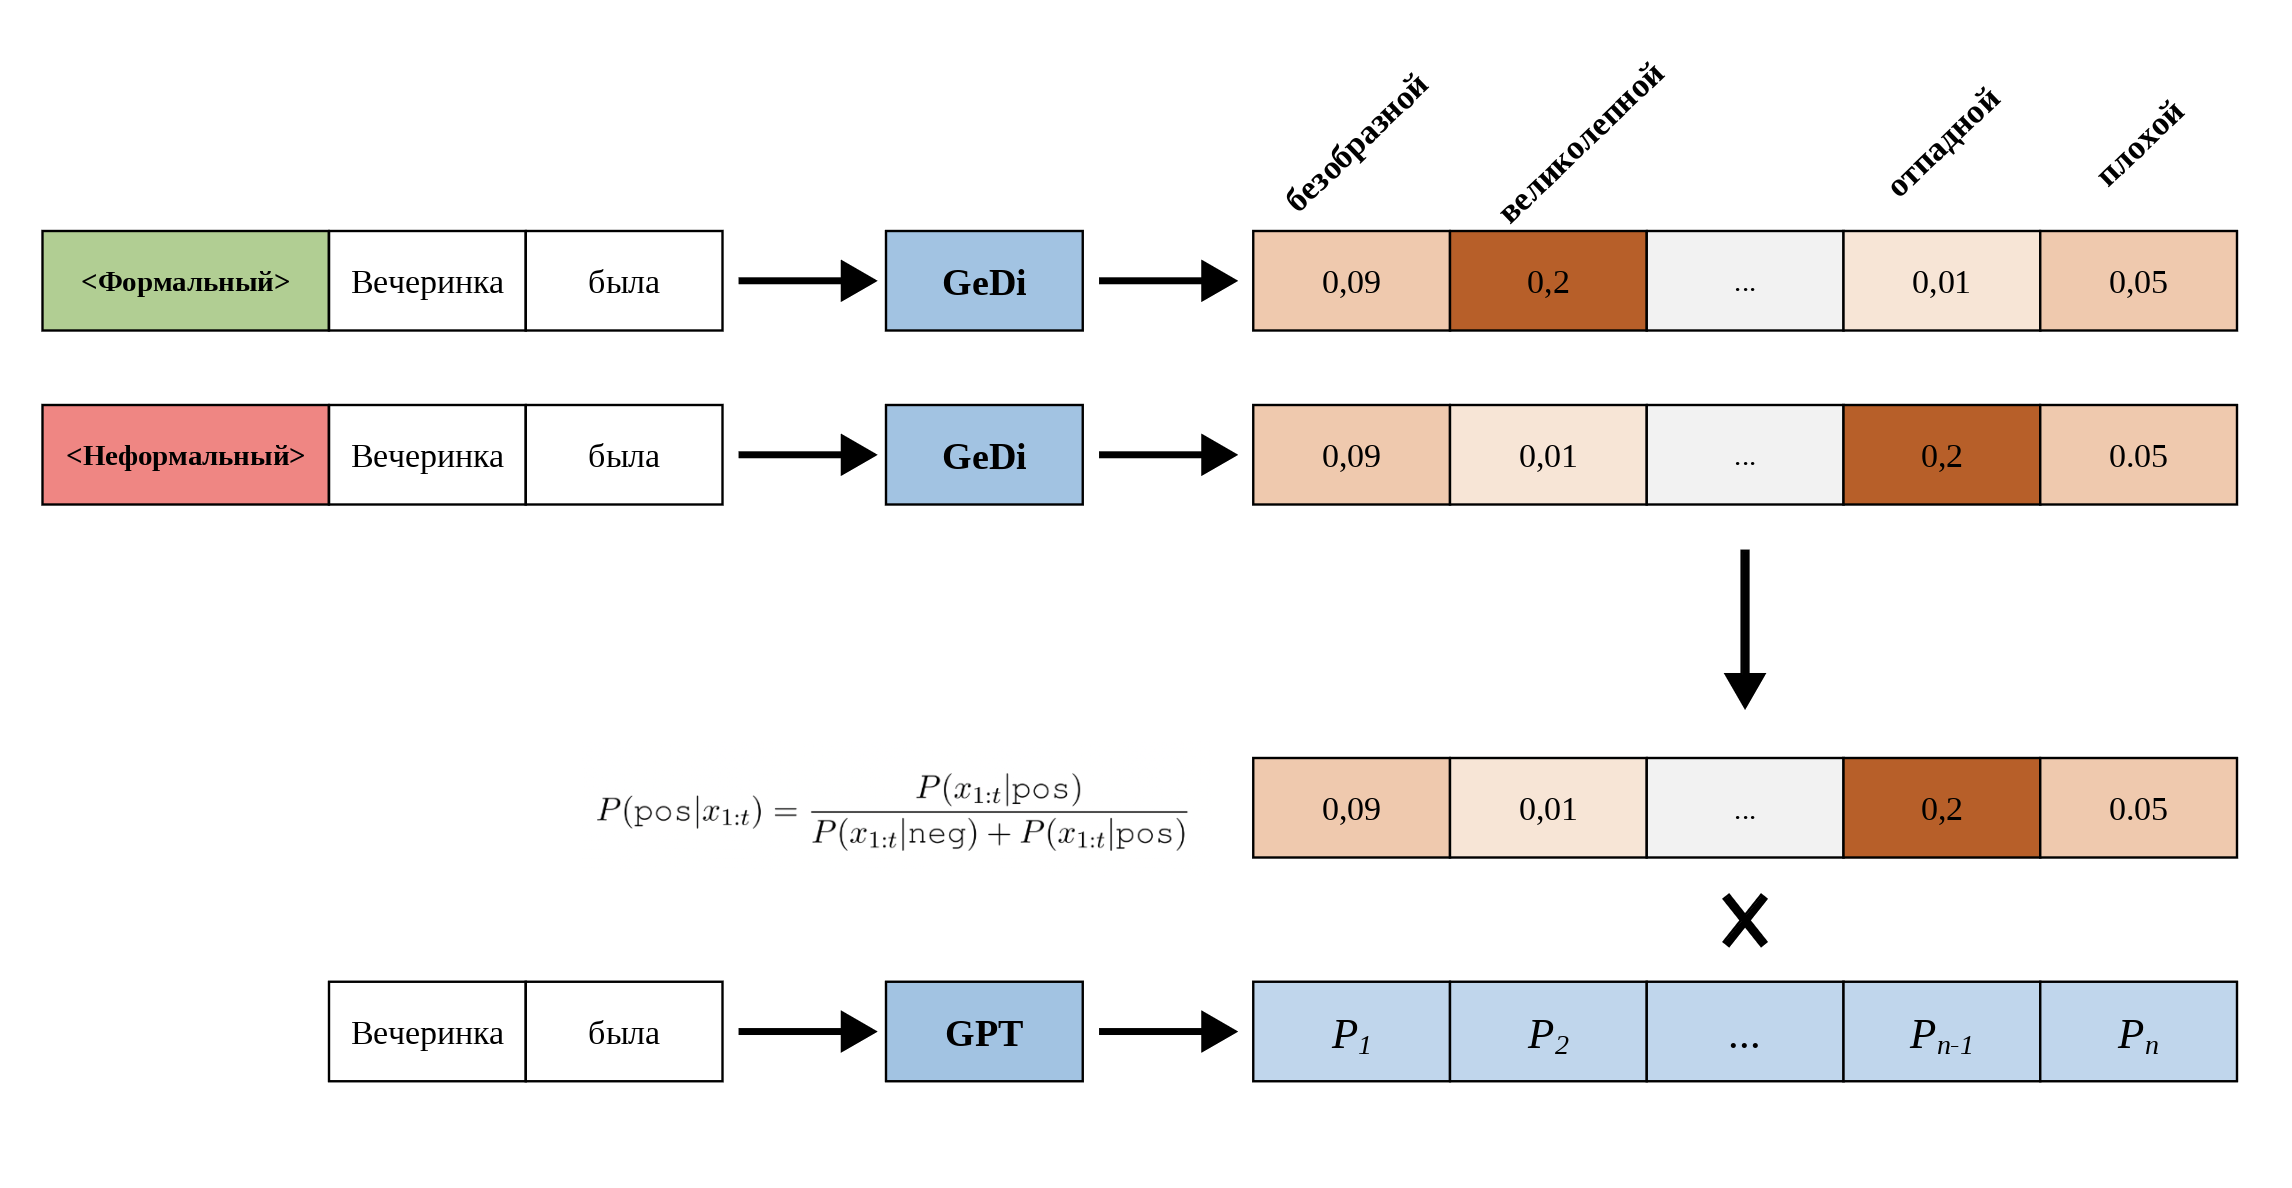
\includegraphics[width=1.0\textwidth]{figures/gedi_original.png}}
  \caption{Модель GeDi}
  \label{fig:gedi_original}
\end{figure}

Чтобы сохранить содержание предложения в работе \cite{dale2021text} предлагается заменить основную языковую модель на модель, обученную на генерацию парафраза.
Пусть $x$ это исходное предложение, $T$ длинна сгенерированного текста $y$, а $c$ это желаемый стиль, то предлагаемая модель моделирует следующую вероятность:
$$
P(y_t|y_{<t},x,x) \propto P_{LM}(y_t|y_{<t}, x)P(c|y_t,y_{<t},x)
\approx P_{LM}(y_t|y_{<t},x)P_D(c|y_t,y_{<t})
$$

Последнее это аппроксимация, потому что вероятность класса должна быть обусловленна как $x$, так и $y$.
Однако это приближение, хотя и не является полностью оправданным, позволяет     отделить модель парафраза (которая требует параллельного корпуса для обучения) от модели стиля (которая требует только текстов с метками стиля, не обязательно параллельных).
Общий принцип работы изображен на рисунке \ref{fig:gedi_paragedi}
\begin{figure}[ht]
  \centering
  \frame{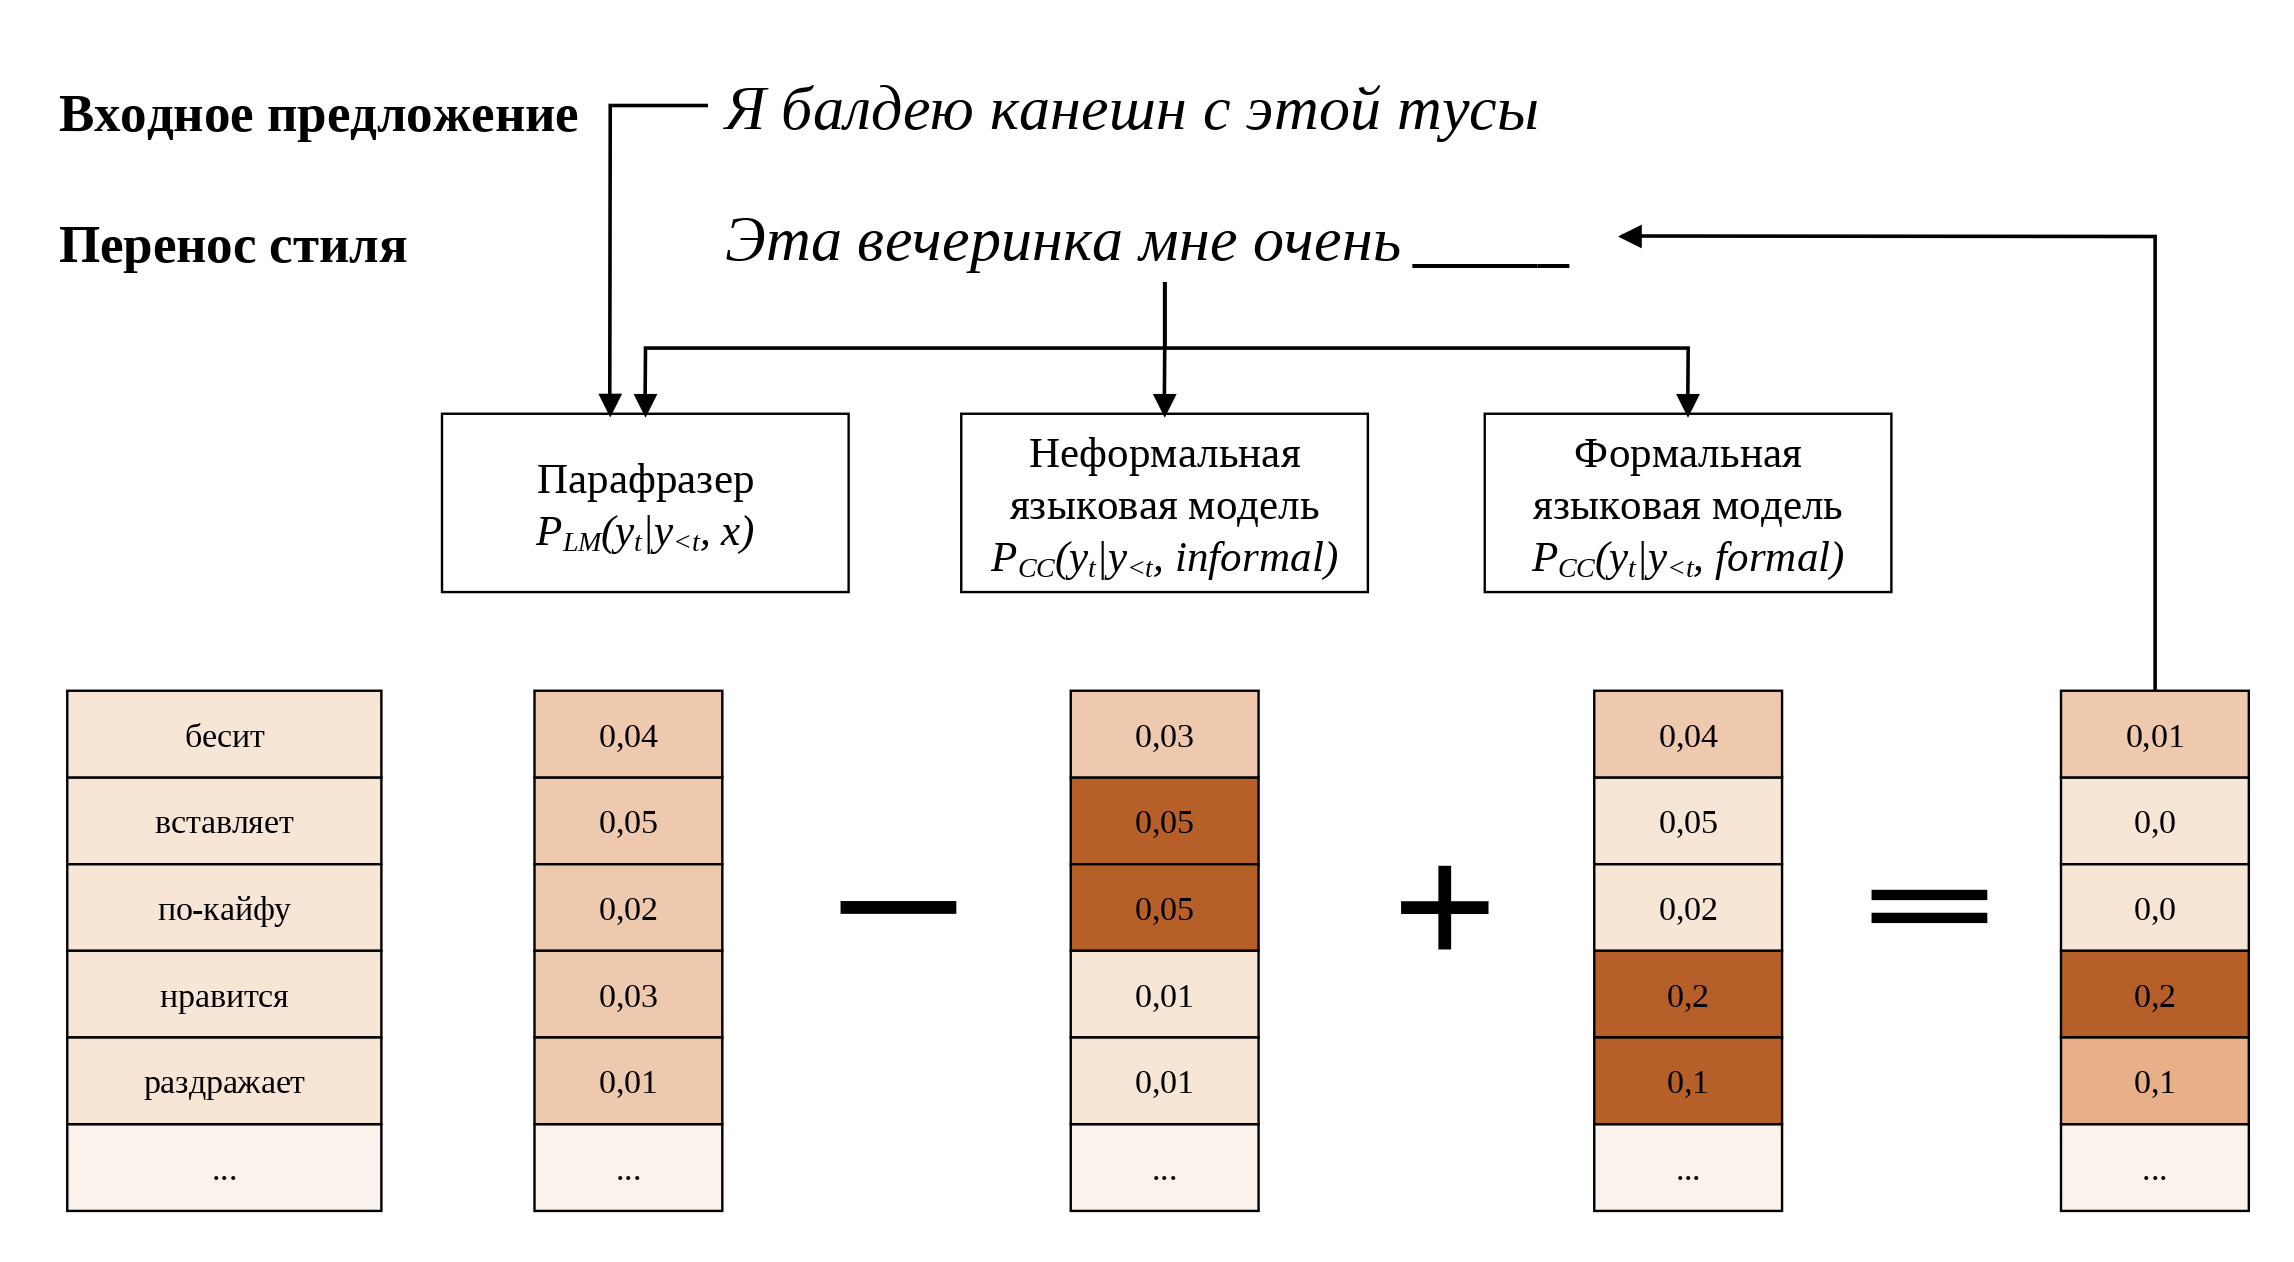
\includegraphics[width=1.0\textwidth]{figures/gedi_detox.png}}
  \caption{Использование модели парафразера в GeDi}
  \label{fig:gedi_paragedi}
\end{figure}

% Обучение
Функция потерь $\mathcal{L}_{ParaGeDi}$ состоит из линейной комбинации двух других функций потерь: генеративной $\mathcal{L}_G$, используемого в обучении языковой модели, и дискриминативной $\mathcal{L}_D$, которая отдаляет разные классы друг от друга в латентном пространстве.
$$
\mathcal{L}_G = - \frac{1}{N} \sum_{i=1}^N 
\frac{1}{T_i} \sum_{t=1}^{T_i} \log P (y_t^{(i)}|y_{<t}^{(i)}, c^{(i)})
$$
$$
\mathcal{L}_D = - \frac{1}{N} \sum_{i=1}^N \log P(c^{(i)}|y_{1:T_i}^{(i)})
$$
$$
\mathcal{L}_{ParaGeDi} = \lambda \mathcal{L}_D + (1 - \lambda) \mathcal{L}_G
$$

В качестве условной языковой модели была использована \texttt{ai-forever/rugpt3large\_based\_on\_gpt2}, а в качестве модели парафраза был взят предобученный \texttt{cointegrated/rut5-base-paraphraser}.

% Результаты и примеры
Метрики качества итогового алгоритма представлены в таблице \ref{table:results}, а примеры генерации в приложении \ref{cha:appendix1}.


% Можно заметить, что задача по переводу из неформального в формальный стиль также оказалась трудновыполнимой, но по сравнению с предыдущим методом был получен прирост в 0,12 по переводу в формальный стиль.

Заметим, что основаные на референсах n-грамные метрики значительно ухудшились, но в то же время можно наблюдать вполне удовлетворительные парафразы.
Здесь стоит сделать вывод и подтвердить другие недавние исследования \cite{li2018delete, mir2019evaluating, shen2022evaluation} о том, что несмотря на наличие параллельного набора данных данные метрики для этой задачи являются не самыми адекватными.
Ведь каждый конкретный стиль может быть выражен разными конструкциями и нет однозначного сопоставления.





\section{Parameter-efficient fine-tuning}
% Общая идея
Параметро-эффективные методы (Parameter-Efficient Fine-Tuning, PEFT) зарекомендовали себя как очень простой и в то же время крайне результативный подход к решению большинства задач.

Общая идея всех методов сводится к:
\begin{enumerate}
    \item использованию больших предобученных языковых моделей (Large Language Models, LLMs);
    \item заморозке всех её параметров;
    \item добавлению небольшого (могут быть десятые доли одного процента от всех параметров) количества дообучаемых параметров;
    \item обучению этих параметров на небольшом наборе данных.
\end{enumerate}

Такой подход даёт следующие преимущества:
\begin{itemize}
    \item если, при наличии набора данных низкого качества, во время классического дообучения (fine-tuning) модель могла ухудшить качество на некоторых задачах, то в этом семействе методов подобного не наблюдается;
    \item значительно снижается необходимое количество размеченных данных – от нескольких сотен до нескольких тысяч примеров;
    \item удобство использования в итоговой системе, потому что достаточно иметь одну большую модель и сколь угодно много адаптеров к ней, которые можно быстро переключать между собой по мере необходимости;
    \item легко дообучать на поступающих новых данных.
\end{itemize}

\subsection{LoRA}
Low-Rank Adaptation of Large Language Models (LoRA) -- метод дообучения, основанный на заморозке весов предобученной модели и добавлении обучаемых матриц ранговой декомпозиции в каждый слой аркитектуры модели, значительно сокращая количество обучаемых параметров \cite{lora}.

Пусть имеется предобученная авторегрессивная языковая модель $P_\Phi(y|x)$, параметризованная $\Phi$.
Каждая задача представлена обучающим набором данных пар контекст-ответ: $\mathcal{Z} = \{(x_i, y_i)\}_{i=1,...,N}$, где оба $x_i$ и $y_i$ представляют собой последовательность токенов.
Во время полноценного дообучения (fine-tuning) модель инициализирована предобученными весами $\Phi_0$ и обновляется как $\Phi_0 + \Delta \Phi$, многократно следуя градиенту для решения максимизационной задачи условного языкового моделирования:
$$
\max_{\Phi}
\sum_{(x,y)\in \mathcal{Z}}
\sum_{t=1}^{|y|}
\log(P_\Phi(y_t|x,y_{<t}))
$$

Основным недостатком является то, что для каждой задачи обучается различный набор параметров $\Delta\Phi$, размерность которого $|\Delta\Phi|$ равна $|\Phi_0|$.
Соответственно, с увеличением размера предобученной модели, хранение и разворачивание множества реплик предобученной модели становится всё более сложной задачей.

В данном подходе применяется более эффективный с точки зрения параметров подход, при котором приращение параметра $\Delta\Phi = \Delta\Phi(\Theta)$ для конкретной задачи дополнительно кодируется набором параметров $\Theta$ гораздо меньшего размера $|\Theta| \ll |\Phi_0|$.
Задача нахождения $\Delta\Phi$ превращается в задачу оптимизации по $\Theta$:
$$
\max_\Theta
\sum_{(x,y)\in \mathcal{Z}}
\sum_{t=1}^{|y|}
\log(p_{\Phi_0 + \Delta\Phi(\Theta)}(y_t|x,y_{<t}))
$$

Нейронная сеть состоит из множества полносвязных слоёв, которые выполняют матричное перемножение.
Матрицы весов в этих слоях обычно являются полноранговыми.
Исследования показывают, что при адаптации к специфической задаче предобученные подели имеют маленькую "`внутреннюю размерность"' и могут эффективно обучаться, несмотря на случайную проекцию в меньшее подпространство \cite{aghajanyan2020intrinsic}.
Из данного наблюдения вытекает гипотеза, что обновления веса моделей тоже имеют небольшую "`внутреннюю размерность"'.
Для предобученной матрицы весов $W_0 \in \mathbb{R}^{d \times k}$ ограничивается её обновления, представляя его в виде разложения низкого ранга $W_0+\Delta W = W_0 + BA$, где $B \in \mathbb{R}^{d \times k}, A\in \mathbb{R}^{r \times k}$ и ранг $r \ll min(d,k)$.
Во время обучения матрица $W_0$ заморожена и не получает обновлений от градиента, в то время как $A$ и $B$ являются обучаемыми параметрами.
Оба $W_0$ и $\Delta W = BA$ умножаются на одинаковый вектор, а их соответствующие выходные вектора по-координатно суммируются.
Для $h = W_0 x$ модифицированный прямой проход:
$$h = W_0x + \Delta W x = W_0x + BAx$$
Данное выражение изображено на рисунке \ref{fig:lora}.
Для $A$ используется случайная Гауссова инициализация, а $B$ инициализируется нулями, так что $\Delta W = BA$ равна нуля в начале обучения.

\begin{figure}[ht]
  \centering
  \frame{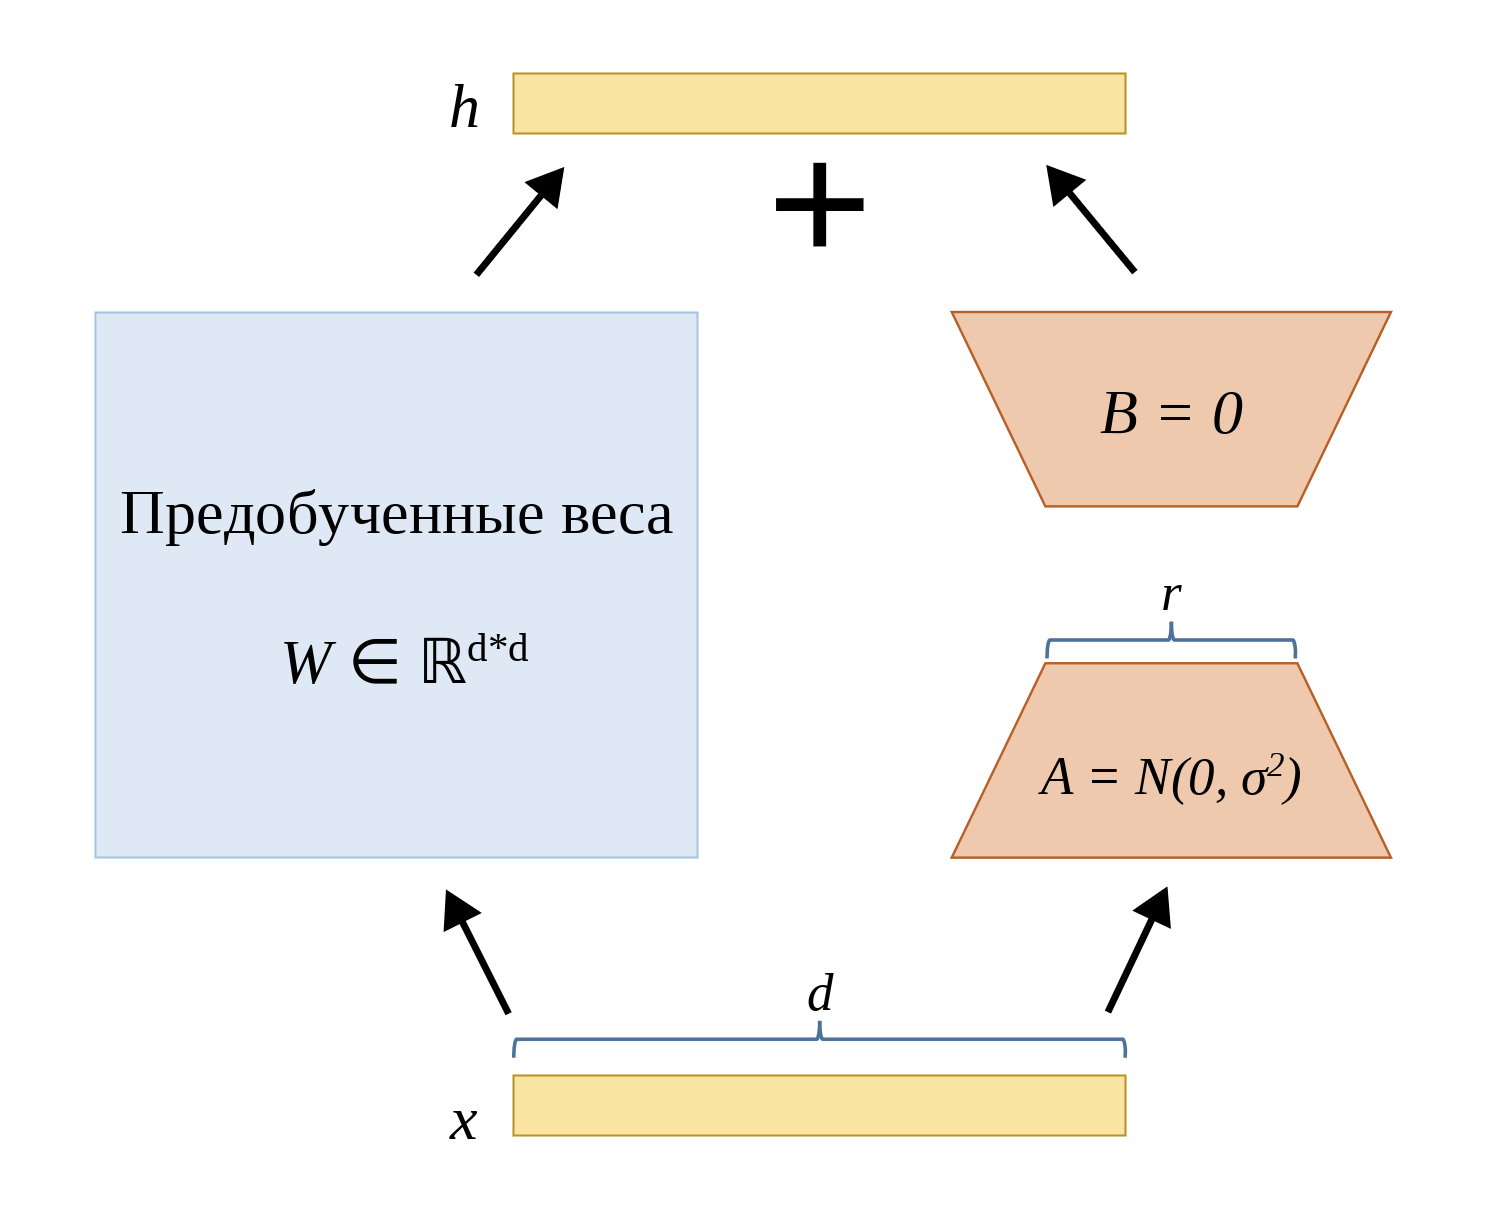
\includegraphics[width=0.7\textwidth]{figures/lora.png}}
  \caption{Параметризация весов в алгоритме LoRA. Обновляются только матрицы $A$ и $B$}
  \label{fig:lora}
\end{figure}

В работе с помощью данного алгоритма была дообучена модель \texttt{cointegrated/rut5-base-paraphraser} на собранном наборе данных.
Метрики качества указаны в таблице \ref{table:results}, а примеры генерации в  в приложении \ref{cha:appendix1}.


\subsection{P-Tuning}
Данный метод основан на автоматическом поиске затравок (prompts) в непрерывном пространства \cite{gpt_understands_too}.

Пусть дана предобученная языковая модель $\mathcal{M}$.
Последовательность дискретных входных токенов 
$x_{1:n} = \{x_0, x_1, ..., x_n\}$
будет сопоставлена с входными эмбеддингами 
$\{\mathbf{e}(x_o), \mathbf{e}(x_1), ..., \mathbf{e}(x_n)\}$
с помощью предварительно обученного слоя ембеддингов
$\mathbf{e} \in \mathcal{M}$.
В конкретном случае, зависящем от контекста $\mathbf{x}$, часто используются выходные эмбеддинги набора целевых токенов  $\mathbf{y}$ для последующей обработки.

Функция затравки (промпта) $\mathbf{p}$ - организовать контекст $\mathbf{x}$, результат $\mathbf{y}$ и саму себя в шаблон $T$.
Для задачи переноса стиля текста шаблоном может быть "<Перепиши предложение "`$\mathbf{x}$"' в неформальном стиле: "`$\mathbf{y}$"'">.
Здесь "<Перепиши предложение ... в неформальном стиле: ..."> это затравка, $\mathbf{x}$ это контекст, а $\mathbf{y}$ это результат.

Пусть $\mathcal{V}$ это словарный запас языковой модели $\mathcal{M}$, а $[P_i]$ является $i$-ым токеном шаблона $T$.

Имея шаблон $T = \{ [P_{0:i}],x,[P_{i+1:m}], y \}$, дискретная затравка удовлетворяет условию $[P_i] \in \mathcal{V}$ и превращает $T$ в
$$\{ \mathbf{e}([P_{0:i}]), \mathbf{e}(\mathbf{x}), \mathbf{e}([P_{i+1:m}]),\mathbf{e}(\mathbf{y}) \}$$

В отличии от этого, P-tuning воспринимает $[P_i]$ как псевдо-токены и превращает шаблон в
$$\{h_0, ..., h_i, \mathbf{e}(\mathbf{x}), h_{i_1}, ..., h_m, \mathbf{e}(\mathbf{x})\}$$
где $h_i(0 \leqslant i < m)$ это обучаемые эмбеддинги.
Это позволяет находить лучшие непрерывные затравки вне словарного запаса, которым оперирует языковая модель.
Сравнение дискретного поиска и P-tuning приллюстрировано на рисунке \ref{fig:p_tuning}.

Имея функцию потерь $\mathcal{L}$ можно дифференциально оптимизировать непрерывные затравки $h_i(0 \leqslant i < m)$ как
$$\hat{h}_{0:m} = \arg\min_h \mathcal{L} (\mathcal{M}(\mathbf{x},\mathbf{y}))$$

\begin{figure}[ht]
  \centering
  \frame{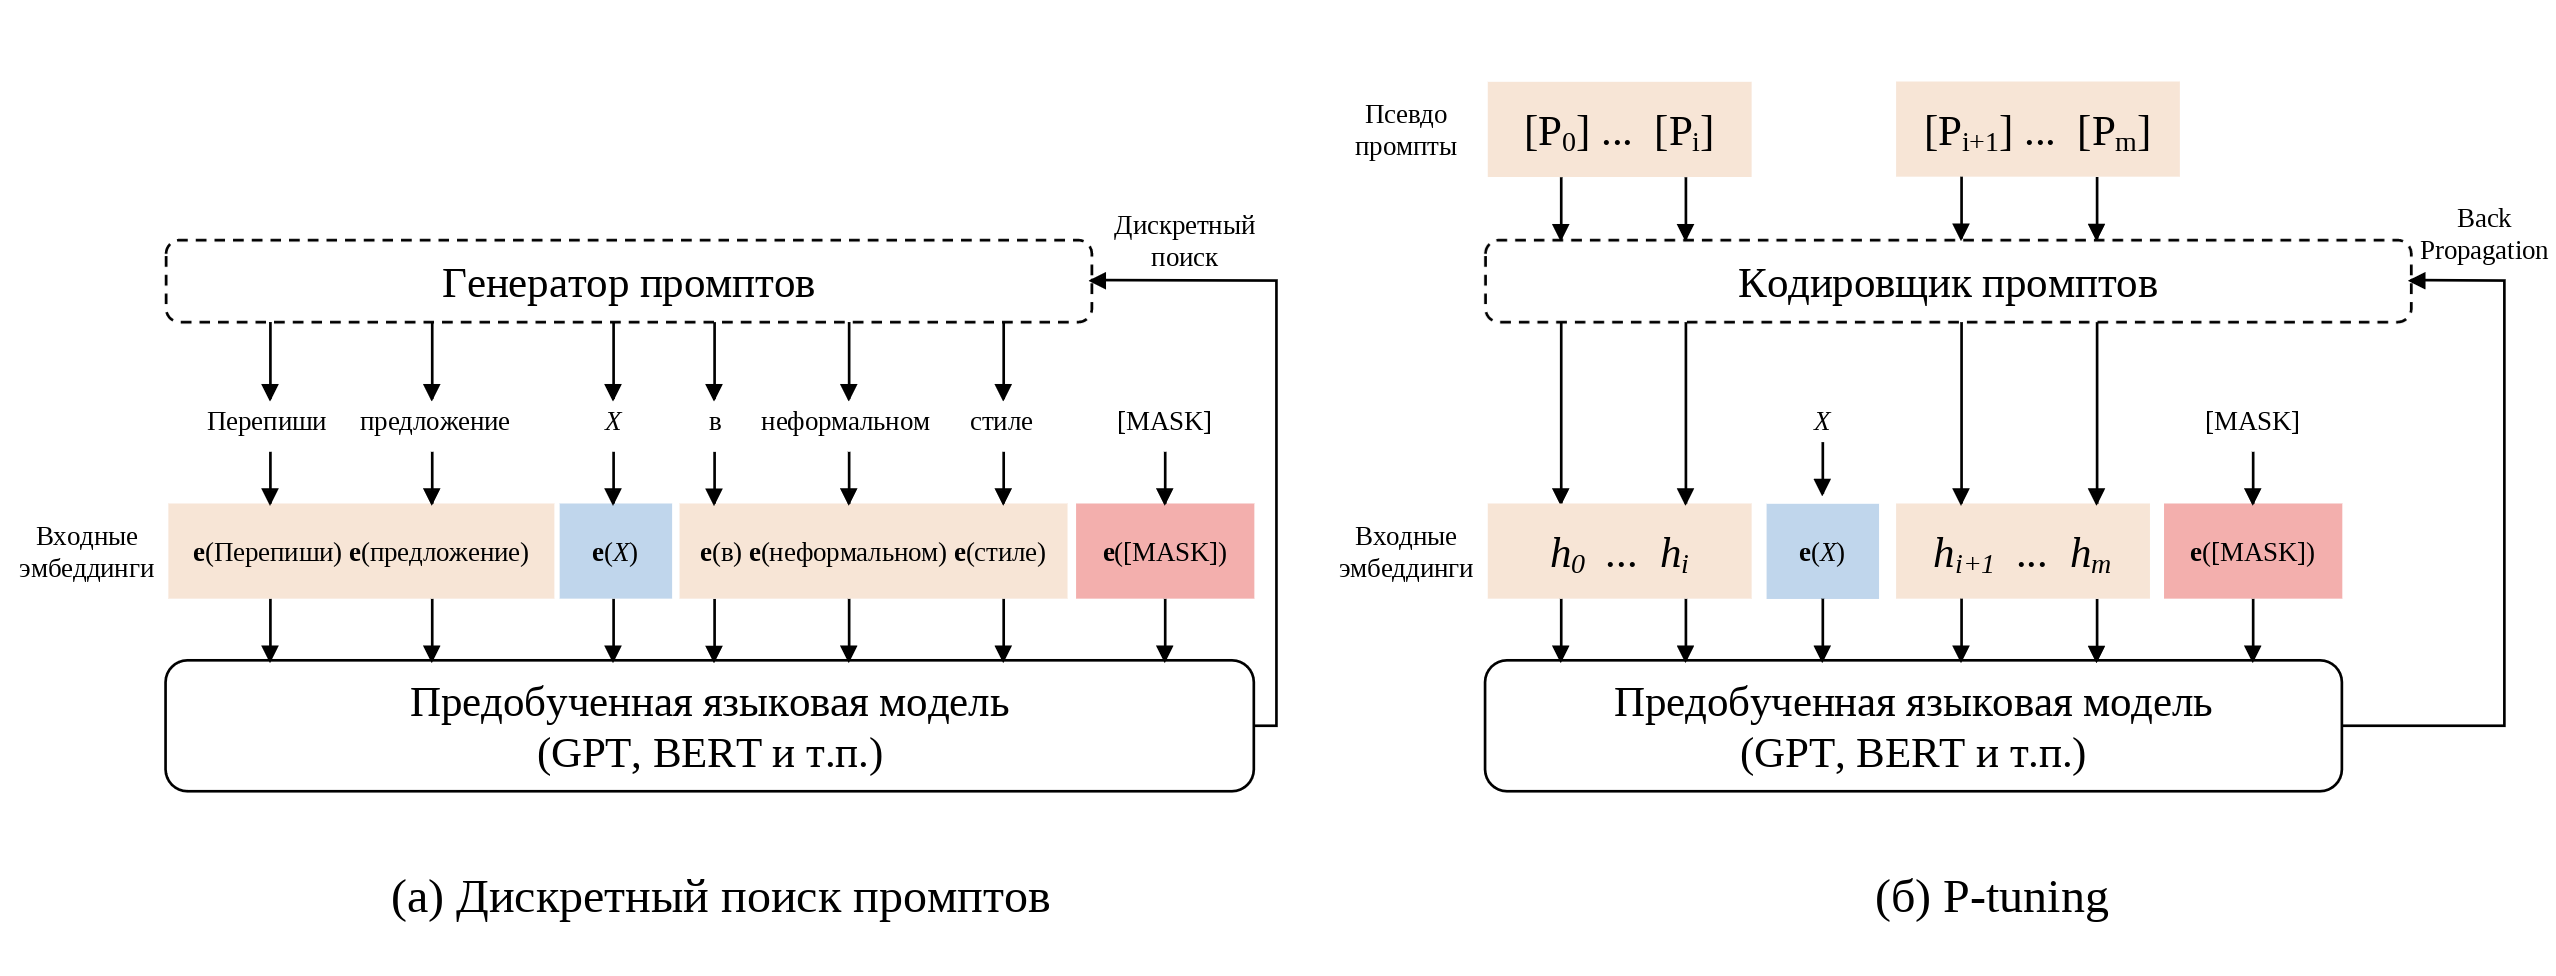
\includegraphics[width=1.0\textwidth]{figures/p_tuning.png}}
  \caption{P-tuning}
  \label{fig:p_tuning}
\end{figure}

В работе с помощью данного алгоритма была дообучена модель \texttt{ai-forever/rugpt3small\_based\_on\_gpt2} на собранном наборе данных.
Метрики качества указаны в таблице \ref{table:results}, а примеры генерации в  в приложении \ref{cha:appendix1}.

\section{Few-Shot LLM}
Появление таких больших генеративных языковых моделей, как ChatGPT и GPT-4 \cite{gpt3, openai2023gpt4} показало, что после превышения определённого числа параметров модель становится достаточно большой, чтобы решать большинство задач во few-shot или даже zero-shot режиме.

В данной работе так же был исследован вопрос, как хорошо справится подобная модель с задачей переноса стиля текста.
Для этого была выбрана модель GPT-4 от OpenAI.
Была подобрана затравка с несколькими примерами изменения формальности текста и модели было дано задание по этому подобию изменить формальность других предложений.
Пример затравки и генераций представлен в приложении \ref{cha:appendix1}.
Можно сделать вывод, что GPT-4 полностью справился с поставленной ему задачей.


\section{Результаты}
Результаты метрик по всем проведенным экспериментам представлены в таблице \ref{table:results}, а примеры генераций в приложении \ref{cha:appendix1}.

Можно сделать вывод, что лучше всего показали себя большие языковые модели, способные без какого-либо дообучения на конкретную задачу показывать результат лучше, чем целенаправленно обученные на задачу модели.
Языковые модели прошлого поколения (GPT-3, T-5 и пр.) с помощью параметро-эффективных методов обучения могут показать хороший результат, особенно в случае отсутствия большого набора данных.
Более старые алгоритмы показывают качество генераций намного хуже.

Обучение без учителя и Guided Generation показали лучшие метрики SacreBLEU и METEOR.
Использование предобученных языковых моделей в сочетании с параметро-эффективными методами дообучения и использование собранного параллельного набора данных дало наилучший результат с точки зрения комбинации метрик Style Score и Semantic Score.
Это подтверждает другие исследования \cite{li2018delete, mir2019evaluating}, что использование метрик, основанных на n-граммах и сравнении с референсами, зачастую не даёт адекватной оценки качества алгоритма.

\begin{table}[ht]
\small
\centering
\caption{Метрики качества исследованных подходов}
\label{table:results}
\begin{tabular}{|p{0.35\textwidth}|c|c|c|c|}
\hline
% \multicolumn{4}{c}{wiki --> lurk / lurk --> wiki}
% Метод & SacreBLEU & METEOR & StyleScore & SemanticScore   \\ \hline \hline
\multirow{2}{*}{Метод} & SacreBLEU & METEOR & StyleScore & SemanticScore   \\ \cline{2-5}
 & \multicolumn{4}{c|}{wiki $\rightarrow$ lurk / lurk $\rightarrow$ wiki} \\ \hline \hline
Unsupervised DAE & 40,5/38,8 & 0,6/0,59 & 0,22/0,6 & 0,82/0,78 \\\hline
Guided Generation & 12,7/6,7 & 0,35/0,27 & 0,13/0,72 & 0,81/0,75 \\\hline
LoRA(ruT5-paraphraser) & 3,04/3,35 & 0,25/0,26 & 0,3/0,75 & 0,79/0,8 \\\hline
P-Tuning (GPT) & 3,16/4,56 & 0,23/0,23 & 0,56/0,92 & 0,73/0,78 \\\hline
\end{tabular}
\end{table}

Также обратим внимание, что с точки зрения StyleScore задача трансфера стиля из формального вики в неформальный лурк является намного более сложной задачей, с которой во всех рассмотренных методах наблюдаются трудности.
Как было упомянуто в параграфе \ref{cha:analysis:sec:datasets} перефразирование в неформальный стиль является более трудной задачей даже для человека.
Стилистическая специфика лурка более сложна и модели труднее её выучить, нежели формальный стиль Википедии.


% \begin{equation}
%     \frac{i + s + d}{n},
%     \label{lev_eq}
% \end{equation}
% \par где $i$ -- количество вставок;
% \par $s$ -- количество замен;
% \par $d$ -- количество удалённых символов;
% \par $n$ -- количество символов/слов в целевой последовательности.

\label{cha:future}
\chapter{Развитие работы}

\section{Продолжение создания набора данных}
% С получением опыта и понимания специфики создания подобного набора данных, имеет смысл продолжить его сбор.
Приняв во внимания аспекты из главы \ref{cha:dataset}, а так же усовершенствование алгоритмов классификации, имеет смысл продолжить создание набора данных на новом качественном уровне.
Усовершенствованные алгоритмы позволят более качественно фильтровать изначальный корпус и выдавать асессорам более качественные предложения.
Тем временем, улучшая взаимодействие с асессорами, можно добиться более высокого итогового качества.

\section{Улучшение метрик качества}
Как было упомянуто в главе \ref{cha:experiments}, данная работа подтвердила другие недавние исследования, указывавшие на проблему соответствия автоматических метрик человеческим оценкам в общем, и в использовании референсных метрик в частности.
Существующие ограничения метрик оценки качества мотивируют к изучению новых способов оценки качества работы моделей по переносу стиля текста.

\section{Улучшение алгоритмов}
Исследование показало, что сбор набора данных хоть и посильная, но очень труднозатратная активность.
В связи с этим дальнейшее изучение и улучшение алгоритмов, не требующих параллельного набора данных, является перспективным направлением.
Особенно в рамках использования больших языковых моделей, показывающих впечатляющий результат, без дообучения на конкретную задачу.
Несмотря на это, большие языковые модели являются чрезмерно громоздкими и работа по уменьшению их размера для использования в задаче переноса стиля текста является обещающим направлением для исследования.


\backmatter %% Здесь заканчивается нумерованная часть документа и начинаются ссылки и
            %% заключение

\Conclusion % заключение к отчёту

% Заключение – последовательное логически стройное изложение итогов исследования в
% соответствии с целью и задачами, поставленными и сформулированными во введении. Заключение
% может включать в себя практические предложения, что повышает ценность теоретического
% материала, но не должно повторять введение
Был собран набор данных для переноса формальности на русском языке объёмом 18 тысяч параллельных пар формальное-неформальное предложение.
Данного набора данных достаточно, для оценки качества моделей, а так же их обучению в случае использования параметро-эффективных методов обучения с современными языковыми моделями.

Можно сделать вывод, что лучше всего в решении поставленной задачи показали себя большие языковые модели, способные без какого-либо дообучения на конкретную задачу показывать результат лучше, чем целенаправленно обученные на задачу модели.
Языковые модели прошлого поколения (GPT-2, GPT-3, T-5 и пр.) с помощью параметро-эффективных методов обучения могут показать хороший результат, особенно в случае отсутствия большого набора данных.
Более подздние алгоритмы показывают качество генераций намного хуже.

Обучение без учителя и Guided Generation показали лучшие метрики SacreBLEU и METEOR.
Использование предобученных языковых моделей в сочетании с параметро-эффективными методами дообучения и использование собранного параллельного набора данных дало наилучший результат с точки зрения комбинации метрик Style Score и Semantic Score.
Это подтверждает другие исследования, что использование метрик, основанных на n-граммах и сравнении с референсами, зачастую не даёт адекватной оценки качества алгоритма.
Данное наблюдение поднимает вопрос о необходимости переосмысления подходов к оценке качества алгоритмов переноса стиля.

% TODO ВЫВОДЫ ИЗ ВВЕДЕНИЯ СТРУКТУРИРОВАНО
% Для выполнения поставленной цели, необходимо решить следующие задачи:
% \begin{itemize}
%     \item проанализировать текущее состояние исследуемой области, существующие подходы к решению данной или схожей задачи, имеющиеся наборы данных;
%     были пр
%     \item определить необходимые метрики и критерии оценки качества будущего алгоритма;
%     \item собрать собственный набор данных;
%     \item провести эксперименты для проверки работоспособности выбранных методов на собранном наборе данных;
%     \item сделать выводы на основании полученных результатов;
%     \item сформулировать планы для дальнейшего развития исследования.
% \end{itemize}



% % Список литературы при помощи BibTeX
% Юзать так:
%
% pdflatex rpz
% bibtex rpz
% pdflatex rpz

\bibliographystyle{gost780u}
\bibliography{rpz}

\chapter{Благодарности}
Хочу выразить благодарность людям, помогавшим в выполнении работы:
\begin{itemize}
    \item Марии Пономарёвой -- за научное руководство и критику;
    \item Александре Ивойловой -- за помощь в создании набора данных;
    \item Студентам РГГУ -- за разметку данных.
\end{itemize}

\appendix   % Тут идут приложения

\chapter{Примеры генераций}
\label{cha:appendix1}

\begin{figure}[ht]
\centering
\ttfamily
% \normal
\fbox{%
	\parbox{\textwidth}{
\underline{Lurk}: В разделе "<Интеллектуальная собственность"> периодически раздаются вопли копирастов. \\
\underline{Wiki}: В разделе "<Интеллектуальная собственность"> периодически раздаются вопли сторонников охраны авторских прав. \\
\underline{Lurk $\rightarrow$ Wiki}: В разделе "<Социальная собственность"> периодически раздаются протесты властей \\
\underline{Wiki $\rightarrow$ Lurk}: В разделе *Социальная собственность* периодически раздаются вопли сторонников охраны авторских прав \\
\\
\underline{Lurk}: После многочисленных высказываний об ущербности интернет-юзеров Михалков напилил видеоблог. \\
\underline{Wiki}: После многочисленных высказываний о неполноценности интернет-пользователей Михалков начал вести видеоблог. \\
\underline{Lurk $\rightarrow$ Wiki}: После многочисленных высказываний об недоности интернет-пользователей Иванов напилил видеоблог. \\
\underline{Wiki $\rightarrow$ Lurk}: После многочисленных высказываний о неполноценности недопользователей Мавроди начал вести видеоблог.  \\
\\
\underline{Lurk}: Алсо, пацанчики с шиномонтажа обширно ловят лулзы со срочников. \\
\underline{Wiki}: Также, парни с шиномонтажа обширно смеются над срочниками. \\
\underline{Lurk $\rightarrow$ Wiki}: Также, рассказчики с шиномонтажа обширно ловят значительные запасы со срочников. \\
\underline{Wiki $\rightarrow$ Lurk}: Алсо, парни с шиномонтажа обширно смеются над срочниками.

	}
}
\caption{Примеры генераций метода DAE}
\label{fig:dae_examples}
\end{figure}


\begin{figure}[ht]
\centering
\ttfamily
% \small
\fbox{%
	\parbox{\textwidth}{
\underline{Lurk}: В разделе "<Интеллектуальная собственность"> периодически раздаются вопли копирастов. \\
\underline{Wiki}: В разделе "<Интеллектуальная собственность"> периодически раздаются вопли сторонников охраны авторских прав. \\
\underline{Lurk $\rightarrow$ Wiki}: В рубрике "<Интеллектуальная собственность"> периодические обращения сторонников защиты авторских прав \\
\underline{Wiki $\rightarrow$ Lurk}: В разделе "<Интеллектуальная собственность"> нередко раздаются вопли копирайтеров. \\
\\
\underline{Lurk}: После многочисленных высказываний об ущербности интернет-юзеров Михалков напилил видеоблог. \\
\underline{Wiki}: После многочисленных высказываний о неполноценности интернет-пользователей Михалков начал вести видеоблог. \\
\underline{Lurk $\rightarrow$ Wiki}: В связи с многочисленными сообщениями о некорректности использования Интернета, Михаилков приступил к созданию видео-блога. \\
\underline{Wiki $\rightarrow$ Lurk}: После нескольких высказываний Михалкова о недоверии к интернет-пользовательам, он начал создавать видеоблоги. \\
\\
\underline{Lurk}: Недавно МВД выпустили свой комикс дабы научить личинок и школоту порядку на улице. \\
\underline{Wiki}: Недавно МВД выпустили свой комикс в целях научить детей и школьников порядку на улице. \\
\underline{Lurk $\rightarrow$ Wiki}: Недавно МВД сделали комиксы с целью научить деток порядку. \\
\underline{Wiki $\rightarrow$ Lurk}: "<МВД"> же недавно выпустили комиксы с целью научить школьников к порядке здешней школе.
	}
}
\caption{Примеры генераций метода Guided Generation}
\label{fig:gedi_examples}
\end{figure}



\begin{figure}[ht]
\centering
\ttfamily
% \small
\fbox{%
	\parbox{\textwidth}{
\underline{Lurk}: В разделе "<Интеллектуальная собственность"> периодически раздаются вопли копирастов. \\
\underline{Wiki}: В разделе "<Интеллектуальная собственность"> периодически раздаются вопли сторонников охраны авторских прав. \\
\underline{Lurk $\rightarrow$ Wiki}: Например, в разделе "<Информация о пользователе"> периодически появляются призывы к написанию статей. \\
\underline{Wiki $\rightarrow$ Lurk}: Примерно раз в месяц раздаётся вопиющая *** о том, что авторские права на произведения принадлежат исключительно правообладателям. \\
\\
\underline{Lurk}: После многочисленных высказываний об ущербности интернет-юзеров Михалков напилил видеоблог. \\
\underline{Wiki}: После многочисленных высказываний о неполноценности интернет-пользователей Михалков начал вести видеоблог. \\
\underline{Lurk $\rightarrow$ Wiki}: После нескольких высказалий о недоумении интернет-бользователей, Михалкова начала ведение видеоблога. \\
\underline{Wiki $\rightarrow$ Lurk}: В связи с многочисленными высказываниями об ухудшении интернет-юзеров Михалкова написала видеообзор. \\
\\
\underline{Lurk}: Пост внезапно породил огромное количество обличительных камментов и припоминаний автору его пророчеств и высказываний, спустя сутки сильно стремящиеся к 9000. \\
\underline{Wiki}: Как ни странно, запись спровоцировала огромное количество обличительных комментариев и припоминаний автору его пророчеств и высказываний, спустя сутки сильно стремящихся к бесконечности. \\
\underline{Lurk $\rightarrow$ Wiki}: Пост неожиданно породил большое количество оскорбительных комментариев и воспоминаний автору его предсказаний и высказываниях, через сутки очень стремящимся к 8000. \\
\underline{Wiki $\rightarrow$ Lurk}: Скажем так, запись вызвала колоссальное количество лулзов и припиваний автору его предсказаний и высказываниям, через сутки изрядно стремящимся к бесконечности.
	}
}
\caption{Примеры генераций метода P-Tunning}
\label{fig:ptunning_examples}
\end{figure}


\begin{figure}[ht]
  \centering
  \frame{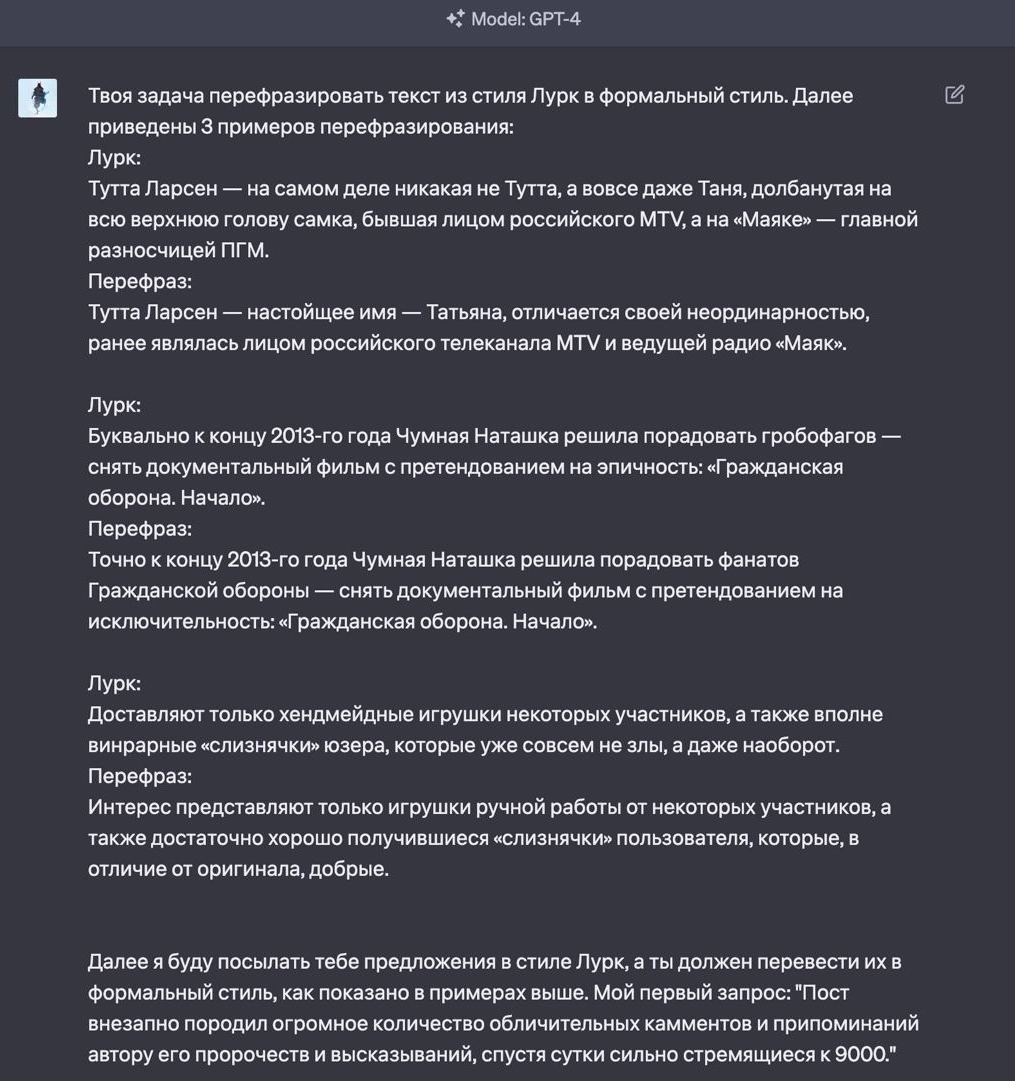
\includegraphics[width=\textwidth]{figures/gpt_lurk2wiki_prompt.jpeg}}
  \caption{Затравка для GPT-4. Неформальный $\rightarrow$ формальный стиль}
  \label{fig:gpt_lurk2wiki_prompt}
\end{figure}

\begin{figure}[ht]
  \centering
  \frame{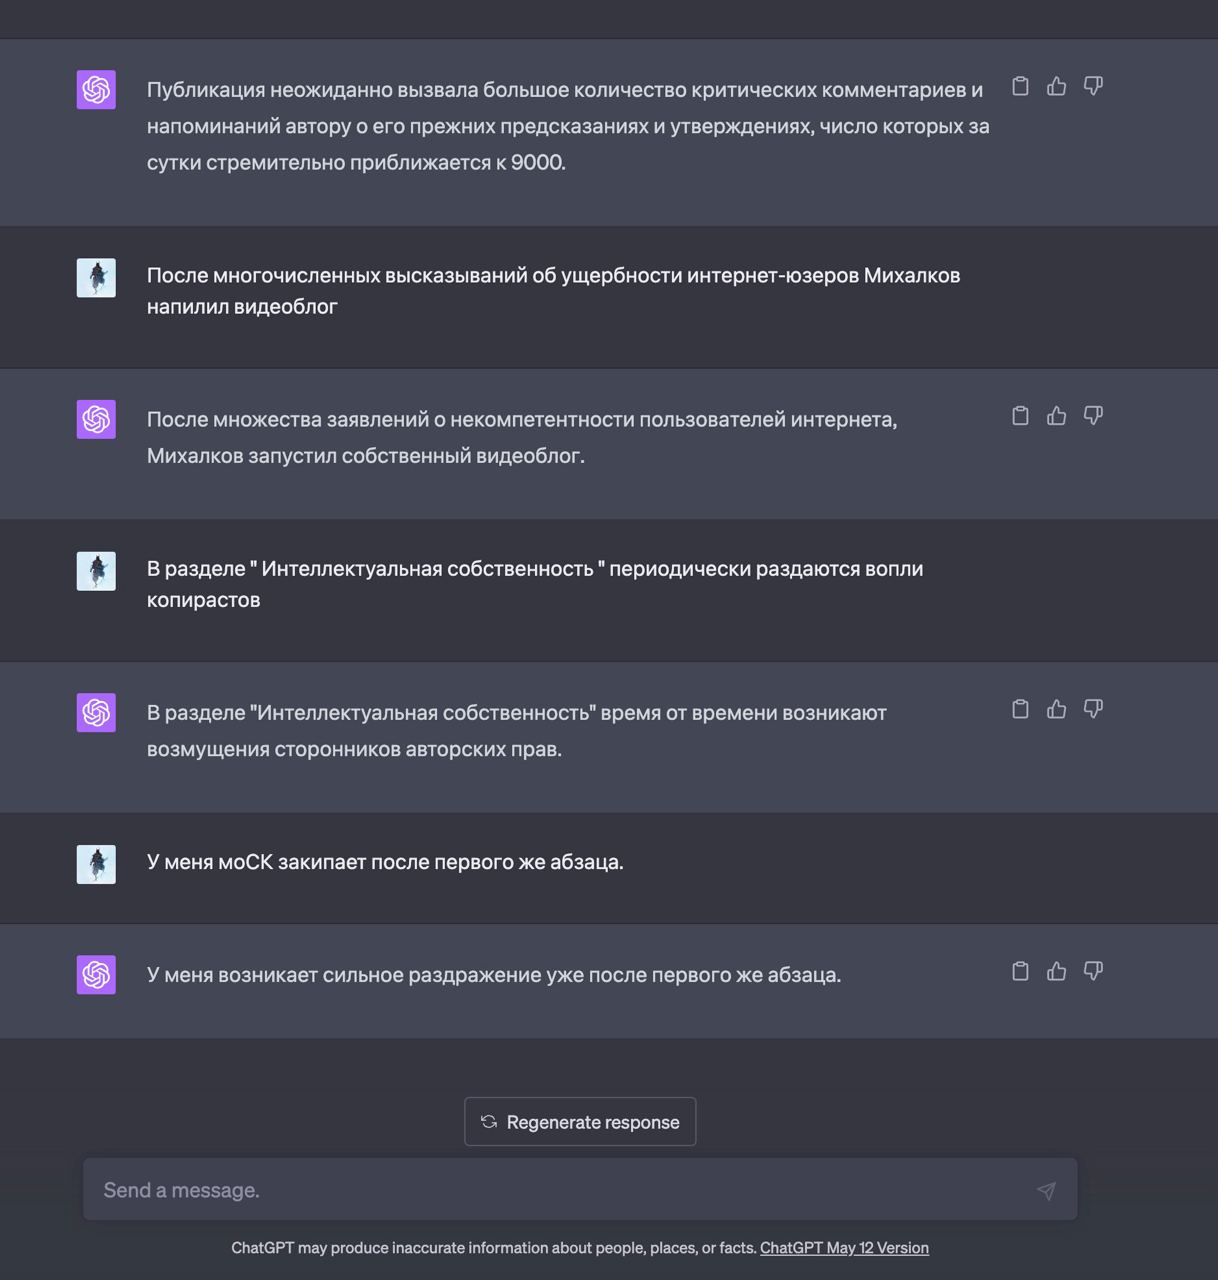
\includegraphics[width=\textwidth]{figures/gpt_lurk2wiki_answers.png}}
  \caption{Ответы GPT-4. Неформальный $\rightarrow$ формальный стиль}
  \label{fig:gpt_lurk2wiki_answers}
\end{figure}

\begin{figure}[ht]
  \centering
  \frame{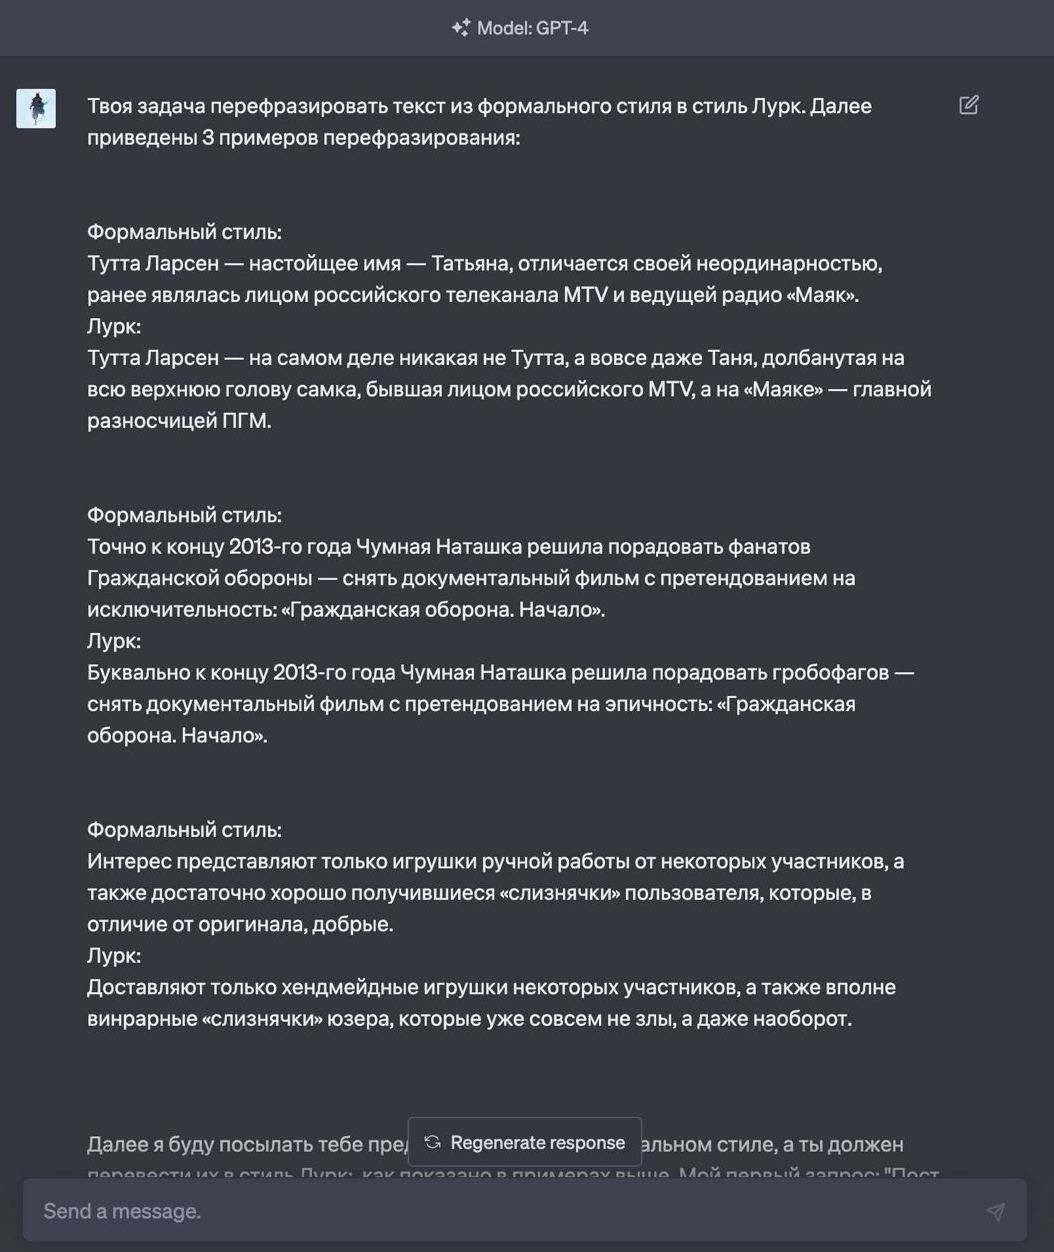
\includegraphics[width=\textwidth]{figures/gpt_wiki2lurk_prompt.jpeg}}
  \caption{Затравка для GPT-4. Формальный $\rightarrow$ неформальный стиль}
  \label{fig:gpt_wiki2lurk_prompt}
\end{figure}

\begin{figure}[ht]
  \centering
  \frame{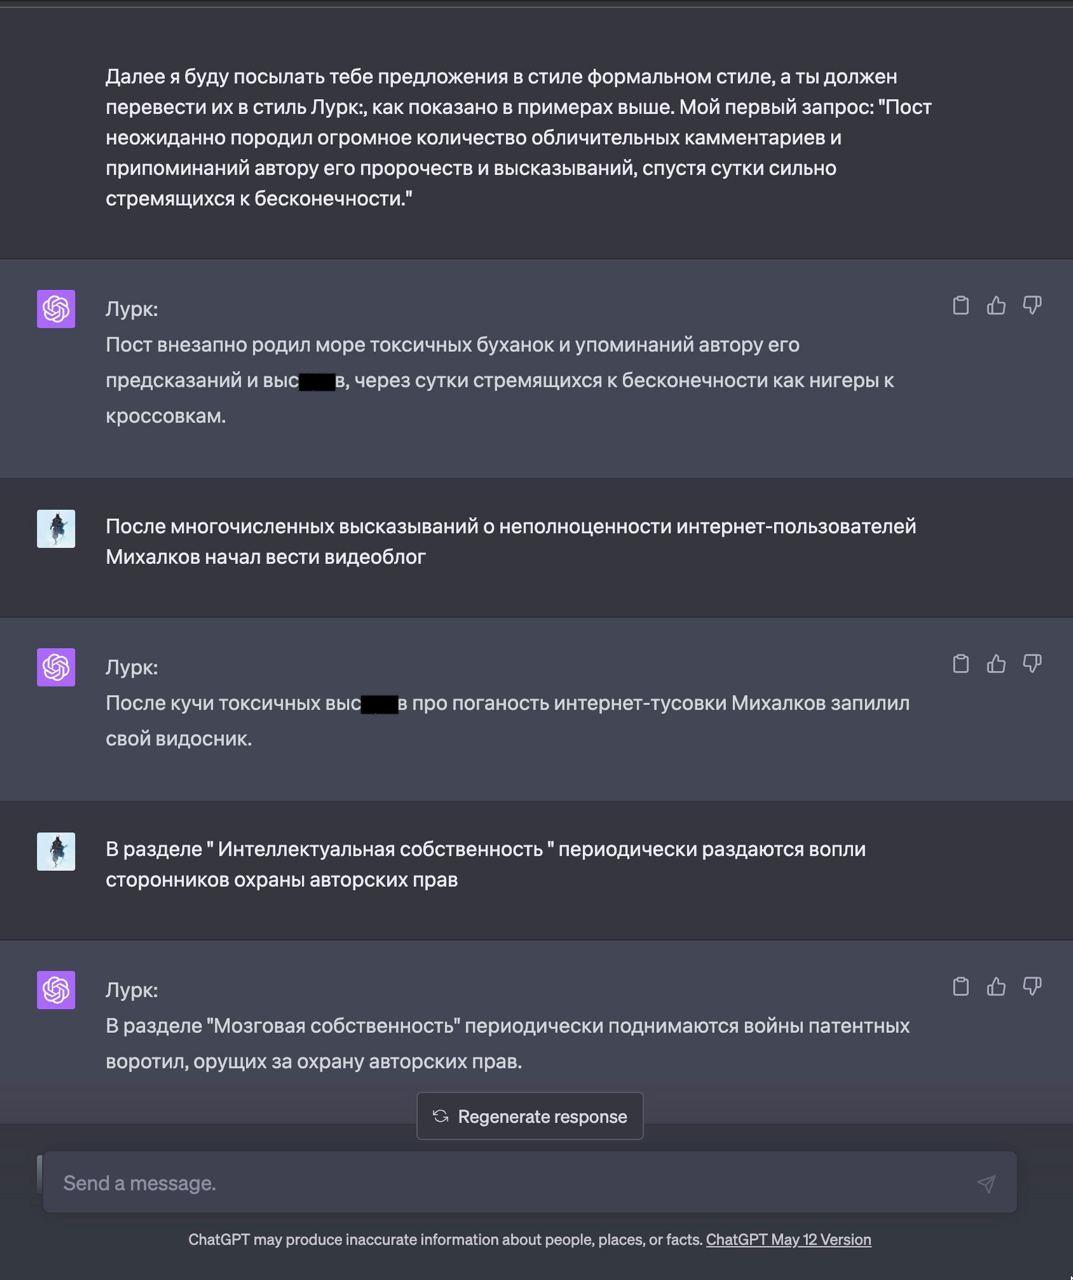
\includegraphics[width=\textwidth]{figures/gpt_wiki2lurk_answers1.jpeg}}
  \caption{Ответы GPT-4. Неформальный $\rightarrow$ формальный стиль}
  \label{fig:gpt_wiki2lurk_answers1}
\end{figure}

\begin{figure}[ht]
  \centering
  \frame{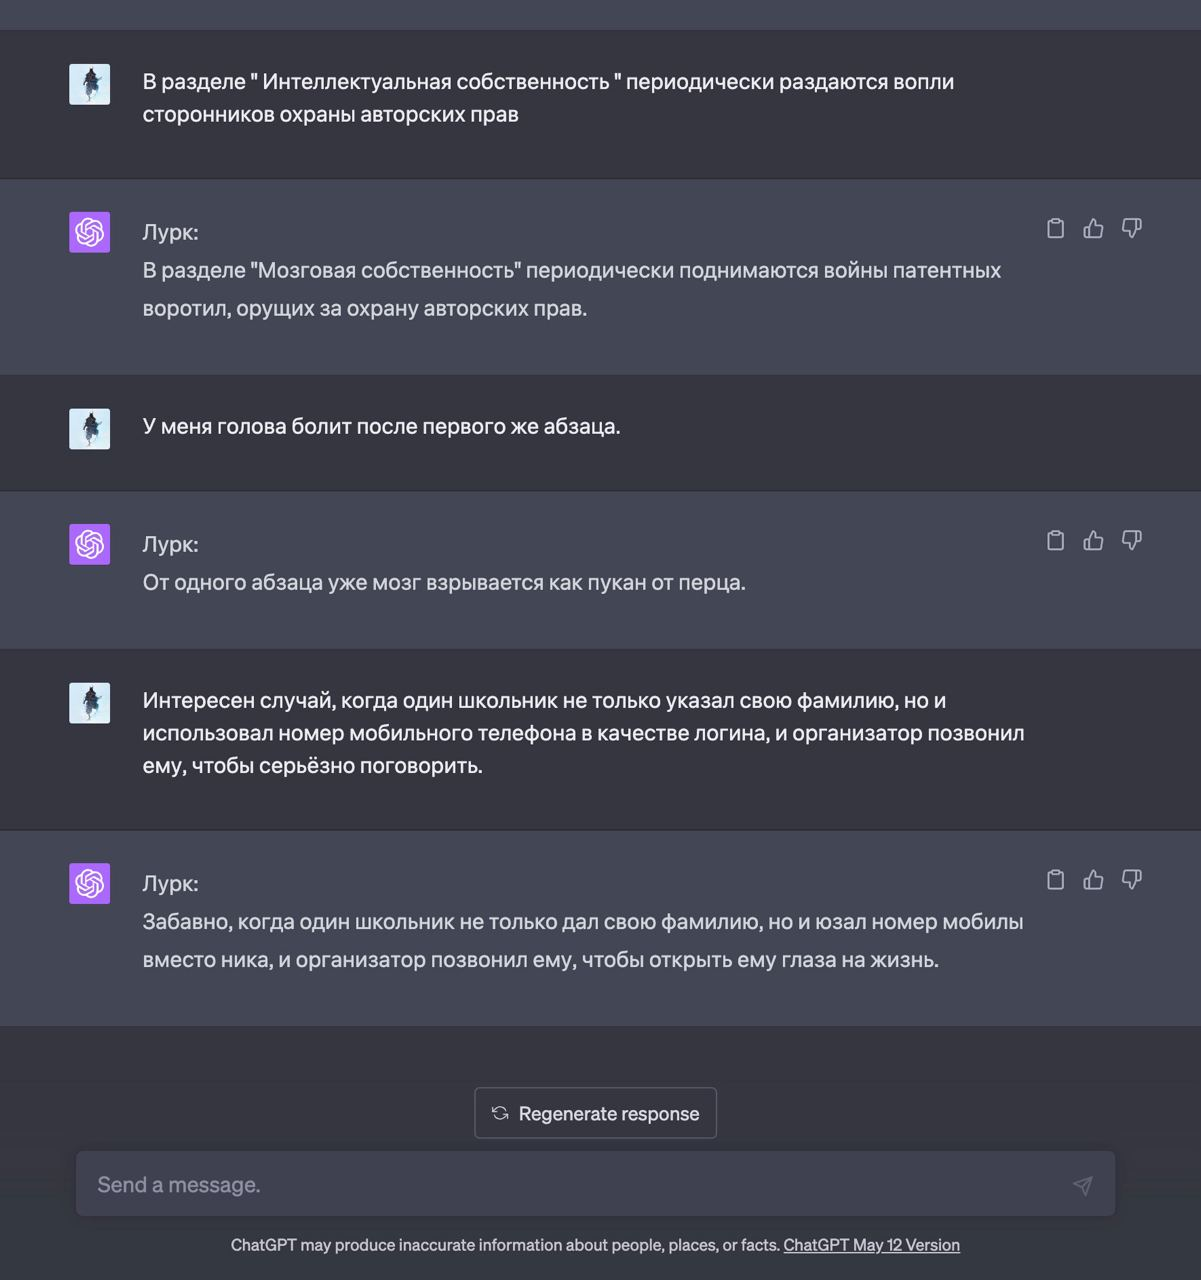
\includegraphics[width=\textwidth]{figures/gpt_wiki2lurk_answers2.png}}
  \caption{Ответы GPT-4. Неформальный $\rightarrow$ формальный стиль}
  \label{fig:gpt_wiki2lurk_answers2}
\end{figure}

\end{document}
